\documentclass[11pt,smallheadings,cleardoublepage=empty,tocflat,numbers=noenddot,twoside,captions=tableheading]{scrbook}
\usepackage[paperwidth=15.5cm,paperheight=22cm,textwidth=11.5cm,textheight=17.2cm,inner=2cm]{geometry}
\usepackage{graphicx}
\usepackage[english]{babel} %% or "american" or "british"
\usepackage[utf8x]{inputenc}
\usepackage[T1]{fontenc}
\usepackage{lmodern}
\usepackage{amsmath}
\usepackage{lipsum} % blind text
\usepackage{comment} % for comment environment
\usepackage{siunitx} % for \num command
\usepackage{float} % for [H] float placement

%% Further packages here:
\usepackage{tabularray} %% recommended for tables
\UseTblrLibrary{booktabs}
\usepackage{expex} %% recommended for linguistic examples

%% The following packages should be loaded last:
\usepackage{microtype}
\usepackage{hyperref}
\hypersetup{
  colorlinks=true,
  linkcolor=black,
  citecolor=black,
  urlcolor=black,
  hyperindex=true,
  linktocpage=true,
}
\urlstyle{same}
%
\usepackage[style=authoryear-comp,backend=biber,natbib=true]{biblatex}
%% standard: \textcite{} and \parencite{}, and \textcites{} and \parencites{}
%% with natbib=true: \citet{} and \citep{}
\addbibresource{references.bib}

\renewcommand{\bottomfraction}{1.0}
\renewcommand{\topfraction}{1.0}
\renewcommand{\textfraction}{0.0}
\emergencystretch4mm
\clubpenalty = 10000 \widowpenalty = 10000 \displaywidowpenalty = 10000

\parskip1ex
\parindent0mm

% alternativ, falls Einzuege statt Abstand gewuenscht
%% \parskip0ex
%% \parindent1.5em

% Moeglicher Kopf fuer Artikel
\newcommand{\chapauthor}[1]{\begin{center}{\large\textsc{#1}}\end{center}\vspace{2ex} \addtocontents{toc}{{\hspace*{1.8mm}\small\textsc{#1}}}}
% kann gern angepasst

% header und footer
\newcommand{\runtitle}{}
\newcommand{\runauthor}{}

\counterwithout{section}{chapter}
\counterwithout{figure}{chapter}
\counterwithout{table}{chapter}
\setcounter{tocdepth}{0}

\usepackage{scrlayer-scrpage}
\lehead[]{\thepage}
\cehead[]{}
\rehead[]{\runauthor}
\lohead[]{\runtitle}
\cohead[]{}
\rohead[]{\thepage}
\lefoot[]{}
\cefoot[\thepage]{}
\refoot[]{}
\lofoot[]{}
\cofoot[\thepage]{}
\rofoot[]{}
\pagestyle{scrheadings}


\begin{document}
\tableofcontents

\cleardoublepage


%%% Authors start here:
\begin{refsection}
\addchap{EnvisionHGdetector: A Computational Framework for Co-Speech Gesture Detection, Kinematic Analysis, and Interactive Visualization}
\chapauthor{Wim Pouw\textsuperscript{1,2},  Sharjeel Ahmed Shaikh\textsuperscript{3,4,5}, James Trujillo\textsuperscript{6}, Bosco Yung\textsuperscript{}, Antonio Rueda-Toicen\textsuperscript{3,4}, Gerard de Melo\textsuperscript{3,4}, Babajide Owoyele\textsuperscript{3,5}}
\renewcommand{\runtitle}{EnvisionHGdetector}
\renewcommand{\runauthor}{Pouw et al.}
{\small
\textbf{Affiliations:}\renewcommand{\thefootnote}{\fnsymbol{footnote}}%
\footnote{Acknowledgments: WP is funded by a DFG VICOM grant (PO 2841/1-1) and an NWO VENI grant (VI.Veni 0.201G.047). WP, GM, and BO are supported by an NWO XS grant (406.XS.24.01.043).}%
\footnote{Contact: \texttt{wim.pouw@donders.ru.nl}, \texttt{Babajide.Owoyele@hpi.de}}%
\renewcommand{\thefootnote}{\arabic{footnote}}%
%
~
\textsuperscript{1}Department of Computational Cognitive Science, Tilburg University, The Netherlands;
\textsuperscript{2}Department of Brain, Cognition and Behaviour, Radboud University, Nijmegen, The Netherlands; 
\textsuperscript{3}Hasso Plattner Institute, Germany; 
\textsuperscript{4}University of Potsdam, Germany; 
\textsuperscript{5}EnvisionBOX team; 
\textsuperscript{6}Institute for Logic, Language and Computation (ILLC), University of Amsterdam, The Netherlands.
}

\textbf{Abstract}. We introduce the \texttt{EnvisionHGdetector} toolkit (v3.1), which allows for the kinematic analysis of automatically detected co-speech gestures from single-person videos. The Convolutional Neural Network (CNN) and Light Gradient Boosting Machine (LightGBM) model for detecting gestures is trained on six open datasets -- ZHUBO, SaGA, MULTISIMO, ECOLANG, TEDM3D, and GESRes -- which, combined, represent over {\color{red}8,000} instances of gestures with varying recording conditions. Inspired and further building on the action detection tool Nodding Pigeon \parencite{yungNoddingPigeonHttps2022}, it utilizes MediaPipe Holistic for skeleton-based tracking, and a CNN/ LightGBM model for classification, running efficiently on CPU only. The tool is designed to work in an out-of-the-box fashion, broadly applicable for any single-person frontal view recording, without custom (p)re-training on specific target datasets. On our test set, we attain an average gesture detection accuracy of 81.2\% with our CNN model and 73.1\% with the LightGBM model. The envisionHGdetector \href{https://pypi.org/project/envisionhgdetector/}{PyPI} package produces as output gesture segment labels, label confidence time series, segmented videos, as well as ELAN files, DTW distance matrices for gesture similarities, kinematic feature summaries, and a data visualization and exploration \href{https://tsg-131-174-75-200.hosting.ru.nl/envisionhgdetectordashboard/}{dashboard}. The code for the package and training is available on \href{https://github.com/WimPouw/envisionhgdetector}{GitHub}, and the training feature data is archived at the \href{https://osf.io/qgecj/}{OSF}. We further discuss this project's outlook, which aims to improve the integration of open-source computational innovations in gesture studies.

\textbf{Keywords:} Co-speech gesture detection, MediaPipe, kinematic analysis, dashboard, machine learning, multimodal communication, gesture studies.

% Introduction
\section{Introduction}
Despite major progress in machine learning and computer vision, and in spite of increasing interest in multimodal aspects of language production, to date, there is no directly applicable co-speech gesture detector designed to work on a variety of recordings of speaking subjects. That is to say, while there is OpenFace for facial gestures \parencite{baltrusaitisOpenFaceOpenSource2016}, OpenPose \parencite{caoOpenPoseRealtimeMultiPerson2021} and MediaPipe \parencite{caoOpenPoseRealtimeMultiPerson2021} for pose detection, OpenSmile \parencite{eybenOpensmileMunichVersatile2010} for speech acoustic feature extraction, there is currently no directly applicable co-speech gesture detector that makes use of current advances in machine learning. The available machine learning methods need to be customized for each unique dataset. In this paper, we introduce the ``Envision Hand Gesture Detector'', a light-weight toolkit for classifying co-speech gestures from video and other actions such as self-adaptors. The toolkit further allows for kinematic analysis and visualization of the detected gestures. The toolkit is available as a PyPI Python package \texttt{EnvisionHGdetector}. Figure~\ref{fig:visual_abstract} provides a visual overview of the EnvisionHGdetector processing pipeline, illustrating the progression from video input to gesture detection and analysis outputs, including the key components of our machine learning approach.

The current limitations to studying gestures on a grand computationally reproducible scale due to the lack of automation stifle the widespread study of human communication in the wild and in the lab. Many scholars are convinced that a better understanding of human hand gestures will provide a deeper understanding of how humans think and what the ultimate format is of their communication \parencite{feyereisenCognitivePsychologySpeechrelated2017, kendonGestureVisibleAction2004,mcneillHandMindWhat1992, goldin-meadowGestureSignLanguage2017, mcneillHandMindWhat1992}. For linguists specifically, understanding gesture means understanding how well-formed aspects of languages are entangled with more imagistic, situated, and pragmatic modes of conveying meaning using a variety of available gestural forms \parencite{alviarMultimodalCoordinationPragmatic2023, murgianoSituatingLanguageRealworld2021}. Such gestural forms include beat gestures, which rhythmically move with prosody of speech \parencite{wagnerGestureSpeechInteraction2014}; they include iconic and metaphoric gestures, which shape to represent something visuo-spatially \parencite{streeckDepictingGesture2008}, and they include a variety of other forms, such as pointing, pragmatic gestures that regulate turn taking, and also emblematic gestures such as a thumbs-up gesture.

To know the difference between scratching your head versus gesturing to simulate scratching your head to signal ignorance is to see a difference that only humans have been able to distinguish and use so far. This is partly because a much broader context must often be considered to differentiate between a gesture and a non-communicative action. Nonetheless, in many cases, the forms that hand movements make when gesturing are quite differentiable from other types of movements and clearly distinct from non-movement. Gestures possess unique rhythms and postures \parencite{pouwEntrainmentModulationGesture2019, streeckDepictingGesture2008, morgensternTheeSingOpening2021}, they exhibit some commonality among people sharing a culture \parencite{kendonGestureVisibleAction2004}, and gestures may, on average, actually diverge from other types of actions, such as scratching the nose, as otherwise gestures would be confusing in their meaning. This is all to say that a machine classifier in the current era of deep learning \parencite{sieversDeepSocialNeuroscience2024} should, in principle, do relatively well in learning to differentiate a gesture from a non-gesture movement, or at least a non-movement. While in principle, there is no reason to believe that machines will ever make a good distinction of something so subtle as the difference between a wink and a blink without taking in a much more elaborate context, for most gestures, it should be relatively straightforward from the form of body movement that it is, in fact, a co-speech gesture. 

\begin{figure}
    \centering
    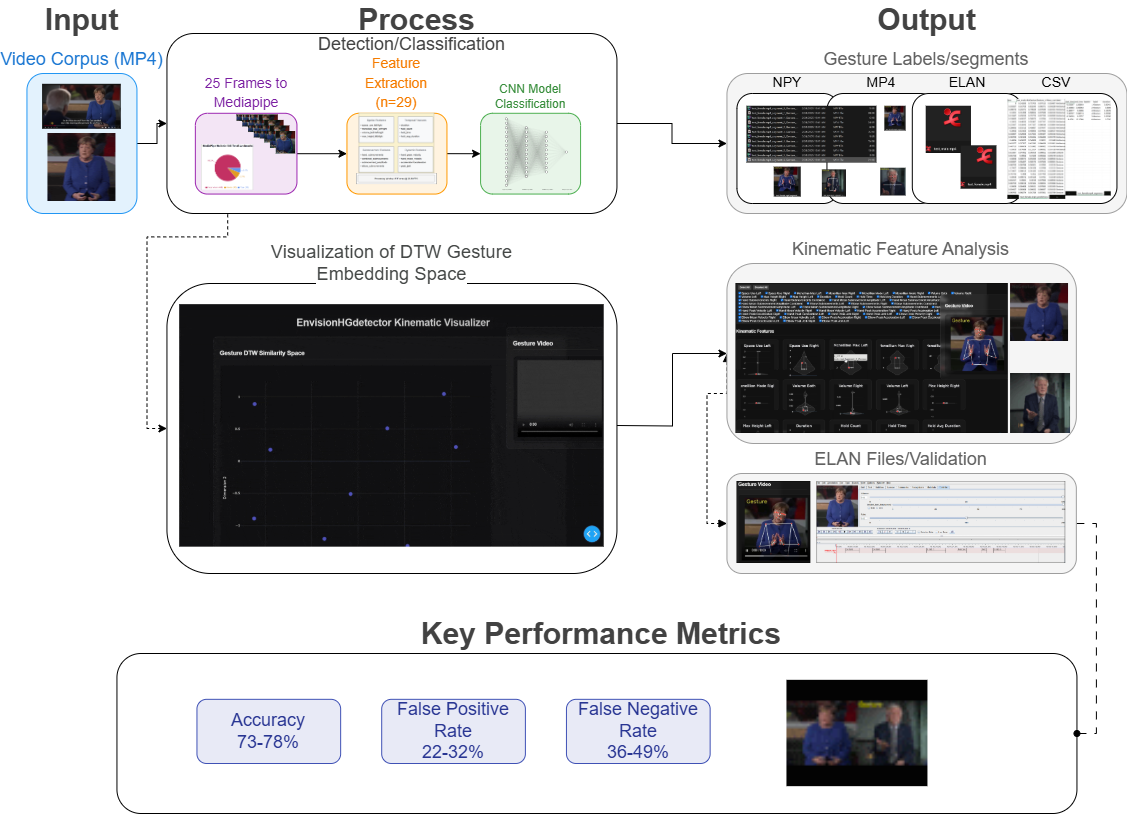
\includegraphics[width=0.8\linewidth]{visual_abstract.png}
    \caption{Video Processing Workflow (Graphical Abstract)}
    \label{fig:visual_abstract}
\end{figure}

To date, there is no such machine learning-based classification tool for co-speech gestures that is directly applicable to videos with variable recording circumstances \parencite{gregoriRoadmapTechnologicalInnovation2023, henleinOutlookAIInnovation2024}, although, as we review below, some successes have been made in co-speech gesture detection. Before going into these successes, we must first emphasize that gesture annotation traditionally requires considerable time and effort. Often, it entails frame-by-frame scrutiny of when a hand starts to move into a meaningful trajectory (known as a stroke phase), which typically requires hours of labour for a single hour of video. Often, multiple annotators are solicited to make such a judgment so as to better assess reliability. Such annotation is challenging to automate, as it requires substantial context that humans implicitly bring along to make their categorizations, for example, when judging an iconic gesture from a beat gesture. However, before such fine-grained distinctions are made, researchers are still annotating for the much simpler distinctions between co-speech gestures and non-gestures.

Research in machine learning is beginning to show that the simpler task of separating gestures from non-gestures in video is increasingly amenable to automation. For example, based on a simple set of rules, you could pre-annotate gestures by assessing the speed time series of hands using pose-tracking and some post-processing \parencite{ripperdaSpeedingDetectionNoniconic2020, eijkCABBDatasetMultimodalundermajorrevision}, as in the OpenPose-based \parencite{caoOpenPoseRealtimeMultiPerson2021} tool SPUDNIG \parencite{ripperdaSpeedingDetectionNoniconic2020}. A problem with rule-based classifiers based on movement is that they often have a high false-positive rate, as any movement is labeled a gesture \parencite{pouwSemanticallyRelatedGestures2021}, reaching false positive rates of 70\% \parencite{ripperdaSpeedingDetectionNoniconic2020} to 86\% \parencite{pouwSemanticallyRelatedGestures2021}. However, the true positive rate sometimes reported is fairly high, often 70\% \parencite{pouwSemanticallyRelatedGestures2021} to $>$99\% \parencite{ripperdaSpeedingDetectionNoniconic2020}. Although these rule-based systems do not differentiate nose-scratching from gesture, they have been shown to speed up gesture annotation via human-in-the-loop quality checking after the first sweep \parencite{ripperdaSpeedingDetectionNoniconic2020}. Of course, with the advent of progress in machine learning, some computer scientists have trained models to make more fine-grained annotations. For example, Ghaleb et al.~\parencite{ghalebCoSpeechGestureDetection2024} trained a state-of-the-art Spatio-Temporal Graph Convolutional
Network (ST-GCNs) to differentiate gesture phases, such as separating the stroke from an optional post-stroke hold. This is a much more difficult task than binary gesture/no gesture classifications because they require discerning subtle differences in kinematics. With this approach, they obtained an accuracy of \textit{61\%} on gesture strokes (with an F1 score of 65.7\%). Other successes have been reported with a tool by Ienega and colleagues \parencite{ienagaSemiautomationGestureAnnotation2022}, which allows a human annotator to train a Light Gradient Boosting Machine on only a portion of hand-annotated gesture labels, so that the classifier can perform the remaining annotation work on the rest of the data. This method was very reliable, and the accuracy was reported to be 86\% (F1-score 84.0\% when 3\% is hand-annotated). There is further an entire subfield of human-computer interaction that is reporting successes in classifying interactive silent stereo-typed gestures \parencite{molchanovOnlineDetectionClassification2016, frontedduDynamicHandGesture2022}, and more generally an interest from the computer science community for the recognition of ``actions'', such as MotionBERT \parencite{zhuMotionBERTUnifiedPerspective2023}. Though not focused on (the possibly more varied) co-speech gestures, such models can very reliably ($>$80\% accuracy) distinguish different types of silent gesture or action classes, and detecting meaningful events from movements underwrites the potential of a general-purpose co-speech gesture classifier.

In light of the above, we can wonder why the reported successes of gesture annotations have not yet translated to the widespread adoption of automatic gesture classification. Nothing stops cognitive scientists from widely training their models for their research annotation needs. We think this has not happened yet on a wide scale because cognitive scientists are not often trained in computer science methods \parencite{sieversDeepSocialNeuroscience2024}, or lack the computational resources to run computer vision tools and high-compute models. In fact, computer programming has only recently become part of most undergraduate curricula in fields such as psychology, albeit still focused on languages such as R, which diverge from most Python-based computer science tools. Additionally, the problem with translating current successes in machine classification of co-speech gestures is that the trained models do not work out-of-the-box for a given dataset, and the different recording conditions and labeling practices diminish the generalizability (and performance metric results) of models that are based on training data from a single corpus or experiment. No real comprehensive open datasets are currently available that can serve as benchmark datasets for classifying co-speech gesture data. However, various open corpora would provide an extensive training dataset when combined and processed to be made machine-readable. Indeed, a more comprehensive, openly available dataset would help the development of a general-purpose out-of-the-box co-speech gesture classifier (see the \href{https://envisionbox.org/multimodaldatasets.html}{EnvisionBOX dataset overview}), similar to tools such as OpenFace \parencite{baltrusaitisOpenFaceOpenSource2016}, which comes equipped with a general-purpose facial gesture classifier, or OpenSmile \parencite{eybenOpensmileMunichVersatile2010}, which provides suites of acoustic features that have been well-tested to capture features important for prosody or emotion-correlated acoustics. As such, there is some road ahead for a thriving field of automatic co-speech gesture classification that can augment the researcher's toolkit or be helpful for social signal processing beyond research (e.g., to help diagnose communication disorders).


To accelerate the translation of computer science advancements to aid cognitive scientists in their study of multimodal communication and vice versa, we here introduce \textit{\textbf{EnvisionHGdetector}}, a toolkit\footnote{While we believe EnvisionHGdetector represents an advance in automated hand gesture detection and computation, we view it as a starting point rather than a final solution. The tool's current capabilities make it immediately useful for many research applications beyond hands, and the open exchange afforded by a forthcoming versatile dataset release (next to the already available feature training data) should provide a foundation for future improvements. We hope this work will contribute to the broader goal of developing more sophisticated computational tools for studying human communication in all its multimodal complexity.} with a general-purpose co-speech gesture classifier trained on multiple datasets, namely SaGA \parencite{luckingBielefeldSpeechGesture2010}, ZHUBO \parencite{baoEditableCoSpeechGesture2024}, TEDM3D \parencite{rohrerTemporalPragmaticAnalysis2022}, ECOLANG \parencite{guECOLANGMultimodalCorpus2025}, MULTISIMO \parencite{koutsombogeraModelingCollaborativeMultimodal2018, koutsombogeraMULTISIMOMultimodalCorpus2017}, and GESRes \parencite{hensel2025richly}. Our package also performs kinematic and similarity analysis, and generates interactive visualizations in the form of a dashboard that links gesture videos with kinematic analysis results as exemplified online.\footnote{\url{https://tsg-131-174-75-200.hosting.ru.nl/envisionhgdetectordashboard/}}

% Method
\section{Method}
\label{sec:methodology}
Our approach combines pose estimation using MediaPipe Holistic with a classifier (CNN/ LightGBM) to detect co-speech gestures, self-adaptors, and non-gesture events. The model was trained on six distinct datasets: SaGA \parencite{luckingBielefeldSpeechGesture2010}, ZHUBO \parencite{baoEditableCoSpeechGesture2024}, TEDM3D \parencite{rohrerTemporalPragmaticAnalysis2022}, ECOLANG \parencite{guECOLANGMultimodalCorpus2025}, MULTISIMO \parencite{koutsombogeraModelingCollaborativeMultimodal2018}, and GESRes  \parencite{hensel2025richly}. These datasets represent diverse recording conditions and relatively diverse speaker styles and language contexts, enhancing the model's generalizability. For easy lookup and download of these datasets, the reader is referred to the EnvisionBOX multimodal datasets overview\footnote{\url{https://envisionbox.org/multimodaldatasets.html}}. {\color{blue} In total, the combined dataset contains 17,089 annotated events, with approximately 48\% being co-speech gestures, 3\% self-adaptors, and 49\% non-gesture events}. Non-gesture events are neutral events randomly sampled from the recordings when no gestures were annotated. They, therefore, consist of sequences of often non-moving poses during conversation or monologue. All videos were processed through MediaPipe Holistic to extract 3D skeletal landmarks, which our classifier used as input features. To ensure evaluation, we employed a cross-validation scheme where all speakers were held out during training, and we further validated on an external sample video that was not similar to the recording contexts of the training data. The following sections detail our data preparation process, model architecture, and training procedure.

{\color{red} Please note that while we introduce and validate the performance of EnvisionHGdetector for version 1.0, which includes the CNN model, we are continuously developing and have already incorporated new features in our version 2.0 that will be validated at a later point. Specifically, we have added functionality of a lightweight gesture tracker, making use of a light gradient boosting machine, which can be used in real-time webcam detection, too. However, this will not be the topic of the current paper.}

\subsection{Dataset: General Approach}
\autoref{tab:envisionhg-datasets} provides the three labels and their distributions we used to train EnvisionHGdetector. All the original datasets have different labels and gesture classification routines; therefore, we collapsed all labels to (co-speech) \texttt{gesture}, \texttt{move}, or \texttt{no-gesture} labels. The \texttt{gesture}
label encompasses all original gesture labels present in any of the source datasets (e.g., \texttt{iconic}, \texttt{beat}, etc.). In contrast, the \texttt{move} label includes self-adaptors and prominent fidgeting (e.g., SaGA's \texttt{move} label, or MULTISIMO's \texttt{N/A} label). The training data contains co-speech gestures produced under Chinese, French, and English spoken languages. Note that we currently do not store or take into account acoustic information in the training (but see \cite{ghalebLeveragingSpeechGesture2024} for possible improvements in gesture detection).

For each dataset, there are only labels for gestures or particular actions. Therefore, no-gesture event videos needed to be created. We achieved this by sampling video segments that did not contain a label, with the segment length being equal to that of a randomly selected gesture event that was also observed for that speaker. In this way, we sampled randomly from time-varying body poses where no labels were present, with the length of the artificial no-gesture label equal to gesture event segment lengths. In all but the SaGA dataset, this was done by sampling at least as many no-gesture events as there were gesture events observed, to keep the data maximally balanced. Only for the SAGA dataset, this was done with relatively fewer no-gesture data. In the future, we aim to fully balance the data contribution during our model training.

\subsubsection{Dataset: Augmentation}
%We further augmented the final training dataset in two ways. First, we
We further augmented the final training dataset. Spcifically, we
doubled the number of videos by mirroring each video along the horizontal axis. With this, we mitigate potential biases in terms of the handedness of the gesture and increase the variability of the data. 

% Table 1: EnvisionHG Categories Table
\begin{table}[htbp]
  \caption{EnvisionHG Categorization by Dataset}
  \label{tab:envisionhg-datasets}
  \centering
  \begin{tblr}{
      width=0.8\textwidth,
      colspec={X[l] X[r] X[r] X[r]},
      row{1} = {font=\bfseries},
      row{7} = {font=\bfseries}
    }
    \toprule
    Dataset & Gesture & Move & No-Gesture \\
    \midrule
    M3D & 749 & 0 & 802 \\
    SaGA & 1,374 & 106 & 1,021 \\
    SaGA++ & 1,729 & 161 & 1,021 \\
    ECOLANG & 7,440 & 0 & 10,185 \\
    ZHUBO & 172 & 0 & 2,242 \\
    MULTISIMO~~ & 2,376 & 540 & 1,286 \\
    GESRes & 2,056 & 28 & 308 \\
    \midrule
    Total & 15,896 & 835 & 15,844 \\

%        M3D & 745 & 0 & 745 \\
%    SaGA & 640 & 54 & 79 \\
%    ECOLANG & 3,740 & 0 & 5,154 \\
%    ZHUBO & 1,390 & 0 & 1,138 \\
%    MULTISIMO & 1,702 & 407 & 1,295 \\
%    GESRes & 2,056 & 28 & 308 \\
%    \midrule
 %   Total & 8,217 & 461 & 8,411 \\
    \bottomrule
  \end{tblr}
\end{table}


% Table 2: Upper Body and Hand Pose Features
\begin{table}[htbp]
  \caption{Extracted Pose Features: Upper Body and Hand Categories}
  \label{tab:pose-features-body-hand}
  \centering
  {\small
  \begin{tblr}{
      width=0.85\textwidth,
      colspec={X[0.18,l] X[0.08,c] X[0.74,l]},
      row{1} = {font=\bfseries},
      cell{2}{1} = {r=8}{l},
      cell{10}{1} = {r=10}{l},
      rowsep=2pt
    }
    \toprule
    Category & ID & Feature Description \\
    \midrule
    Upper Body & 12 & Distance between left and right wrist (norm.) \\
    & 13 & Distance between left and right elbow (norm.) \\
    & 14 & Left elbow to left shoulder distance (norm.) \\
    & 15 & Right elbow to right shoulder distance (norm.) \\
    & 16 & Left wrist to left shoulder distance (norm.) \\
    & 17 & Right wrist to right shoulder distance (norm.) \\
    & 18 & Left shoulder to left ear distance (norm.) \\
    & 19 & Right shoulder to right ear distance (norm.) \\
    \midrule
    Hand Features & 20 & Left thumb to left index finger distance (norm.) \\
    & 21 & Right thumb to right index finger distance (norm.) \\
    & 22 & Left thumb to left pinky distance (norm.) \\
    & 23 & Right thumb to right pinky distance (norm.) \\
    & 24 & X-axis distance: left wrist to left elbow (norm.) \\
    & 25 & X-axis distance: right wrist centered by right elbow (norm.) \\
    & 26 & Y-axis distance: left wrist centered to left elbow (norm.) \\
    & 27 & Y-axis distance: right wrist centered to right elbow (norm.) \\
    & 28 & Left index finger to nose distance (norm.) \\
    & 29 & Right index finger to nose distance (norm.) \\
    \bottomrule
  \end{tblr}
  }
\end{table}

% Table 3: Head and Face Pose Features
\begin{table}[htbp]
  \caption{Extracted Pose Features: Head and Face Categories}
  \label{tab:pose-features-head-face}
  \centering
  \begin{tblr}{
      width=0.9\textwidth,
      colspec={X[0.2,l] X[0.1,c] X[0.7,l]},
      row{1} = {font=\bfseries},
      cell{2}{1} = {r=6}{l},
      cell{8}{1} = {r=5}{l}
    }
    \toprule
    Category & ID & Feature Description \\
    \midrule
    Head Pose & 1 & Head rotation x-axis (up/down) \\
    & 2 & Head rotation y-axis (left/right) \\
    & 3 & Head rotation z-axis (tilt) \\
    & 4 & Nose x-coordinate \\
    & 5 & Nose y-coordinate \\
    & 6 & Nose z-coordinate \\
    \midrule
    Face Geometry & 7 & Base normalization distance (chin to top head) \\
    & 8 & Left eyebrow to left eye distance (normalized) \\
    & 9 & Right eyebrow to right eye distance (normalized) \\
    & 10 & Distance between mouth corners (normalized) \\
    & 11 & Mouth aperture (upper to lower lip distance, normalized) \\
    \bottomrule
  \end{tblr}
\end{table}


\subsection{Datasets: Brief Background}
\subsubsection{SaGA Dataset}
The SaGA (Speech and Gesture Alignment) corpus \parencite{luckingBielefeldSpeechGesture2010} is a multimodal dataset focusing on spatial communication tasks. The original corpus consists of 25 direction-giving dialogues, in which participants (``routers'') describe a virtual reality town environment and a bus route to na\"ive followers after experiencing a virtual bus ride through the town with five landmarks. However, only 6 of these recordings are openly shared online. This spatial communication scenario elicited natural gesture production, as spatial topics are known to prompt frequent gesturing compared to abstract topics \parencite{alibaliGestureSpatialCognition2005}.
The SaGA corpus approaches annotations by combining multiple dimensions. All gestures were segmented to identify stroke phases and classified into combinable categories: beat, deictic, iconic, and discourse gestures. It further contains ''move'' category gestures, which we also adopt, which isolates non-gestural movements such as nose-scratching. Table 1 provides an overview of the gesture labels.

\textbf{Current Usage of SaGA:} From the $N=6$ SaGA corpus videos, we set aside one recording for testing, which means incorporating 640 gesture, 54 move, and 79 no gesture events from five recordings into our training dataset. We further sampled non-gesture events from the same recordings using the random no-gesture event method previously described. 

\subsubsection{MULTISIMO Dataset}
The MULTISIMO corpus \parencite{koutsombogeraModelingCollaborativeMultimodal2018} is a multimodal dataset consisting of recorded interactions between groups of three participants, where two individuals collaborate in solving a quiz, assisted by a facilitator. This structured problem-solving interaction elicited co-speech gestures.

The complete corpus comprises 23 recorded interactions, of which 18 sessions (approximately 3 hours of material) are available for research purposes under a non-commercial license. The recordings are enriched with detailed annotations (e.g, including full speech transcription, laughter type transcriptions), which were not used for our training. Table 1 provides an overview of the gesture labels.

\textbf{Current Usage of MULTISIMO:} For our study, we set aside two interactions for testing, and have incorporated 1,702 gesture labels, 407 moves, and 1,295 no gesture events into our training data.

\subsubsection{ZHUBO Dataset}
The ZHUBO dataset \parencite{baoEditableCoSpeechGesture2024} is a Chinese co-speech gesture corpus specifically designed for gesture synthesis research. The dataset contains 613 videos from 10 news anchors, which means over 10 hours of professional news commentary footage. Each video is approximately 2 minutes long, featuring anchors providing commentary while using professional gestures to enhance their expression. The data includes simple gesture annotations and additional enriched kinematic data: 42 hand keypoints, 33 pose keypoints, and 468 face landmarks extracted using MediaPipe. The data primarily consists of beat gestures that are particularly prominent in this genre, though no such labels were given (only generic gesture labels were given). 

\textbf{Current Usage of ZHUBO:} The training data consisted of 1,390 gestures from ZHUBO, and 1,138 no gesture events.

\subsubsection{TEDM3D Dataset}
The M3D-TED corpus \parencite{rohrerTemporalPragmaticAnalysis2022} is a richly annotated but small multimodal dataset focusing on academic presentations in a conversational style (TED talks), which was primarily developed to exemplify the new multidimensional gesture coding scheme M3D \parencite{rohrerTemporalPragmaticAnalysis2022}. The data consists of over 2 hours of annotated speech and gesture data from native English and French speakers. We only extracted stroke events that were coded according to the MultiModal MultiDimensional (M3D) coding system \parencite{rohrerMultiModalMultiDimensionalM3D}. Accordingly, the gestures were originally categorized along three key dimensions: form (articulator configuration and kinematics), meaning (referentiality and pragmatic function), and prosodic characteristics (phasing, phrasing, and rhythmic properties). For simplicity, we do not report these dimensions separately here \parencite{rohrerTemporalPragmaticAnalysis2022}, and treat the stroke annotations as co-speech gesture labels. Importantly, this TEDM3D dataset is particularly challenging for gesture detection, owing to frame cuts, camera angle changes, and very short and often out-of-frame gestures. As such, this dataset was primarily added to increase the variability of training data. We do think that these videos are too challenging examples and should not be the target data for our classifier.

\textbf{Current Usage of TEDM3D:} We used all data from this dataset to boost training data variability, therefore incorporating all 745 gesture events and 745 no gesture events.

\subsubsection{ECOLANG Dataset}

The ECOLANG corpus provides a multimodal dataset of English, comprising child-directed (38 dyads with 3–4 year-olds) and adult-directed (31 dyads) interactions. The corpus follows a controlled experimental design where participants discuss objects from four categories (tools, animals, musical instruments, food), with three familiar and three unfamiliar objects per category. Object familiarity was determined through caregiver reports for children and normative data for adults. Each dyad completed 30–40 minutes of interaction. In the ``present'' condition, participants could physically interact with objects, while in the ``absent'' condition, they discussed objects from memory. This design systematically captured how communicative behaviors adapt across different referential contexts. The corpus features multimodal annotations, including verbatim speech transcriptions, five distinct gesture categories (representational gestures, pointing, object manipulations, pragmatic gestures, and beat gestures), and eye gaze fixations on objects. Importantly, we do not consider the (co-speech) object manipulations, as they are a very difficult category to handle without accounting for features that relate to the objects being handled. Object interactions further complicate pose tracking and lead to noisy estimates of poses. Thus, we only take gesture labels into account, and no-gesture events that do not overlap with object manipulations (or gestures). Table 1 provides an overview of the original gesture labels.
\textbf{Current usage ECOLANG:} We used the adult-directed interactions only, yielding 3,740 gestures and 5,154 no-gesture events for our training dataset. Given that the ECOLANG data involves many object manipulations that we do not train our model to classify, we will not use ECOLANG for testing. This will, of course, also mean that our model is already limited to be applied to single-person videos that primarily involve conversational settings without object manipulations.

\subsubsection{GESRes Dataset}
The GESRes dataset \parencite{hensel2025richly} is a co-speech gesture corpus that covers three categories (university lecturer, politician, psychotherapist) of speakers engaged in monologue-like speech. The corpus has 12 videos from nine speakers, with video durations ranging from 16 minutes to 48 minutes (in total: 3 hours, 46 minutes). Gestures are coded for type (iconic, metaphoric, emblem, deictic, abstract deictic, beat, adaptor), lexical affiliate, lexeme (a general gesture label), handedness, and several physical properties (e.g., height, radial orientation). The corpus contains videos, annotations, and MediaPipe pose and tracking. 

\textbf{Current usage GESRes:} We included 2,056 gesture events, 308 no-gesture events, and 28 move events in our training data.

\subsection{Model and Training}
Our gesture detection system is built upon the original code base from Nodding Pigeon \parencite{yungNoddingPigeonHttps2022}, where we combine upper body pose estimation with deep learning classification in a two-stage pipeline. For pose features, we adapted the original codebase to utilize MediaPipe Holistic \parencite{lugaresiMediaPipeFrameworkBuilding2019}, which provides tracking of body keypoints, hand landmarks, and facial features. The MediaPipe Holistic framework is ideal for the considered applications due to its high efficiency, working on CPU-only systems, and its comprehensive coverage of full-body landmarks essential for gesture detection.

The classification stage provides 3 options: CNN, LightGBM, and Combined (returning results from both models). CNN employs a 1D convolutional neural network implemented in TensorFlow 2.14. Our architecture consists of three main components: a temporal feature encoder, a spatial feature encoder, and a classification head. The temporal encoder processes sequences of pose keypoints using 1D convolutions to capture motion patterns, while the spatial encoder learns relationships between different body landmarks using 2D convolutions. These features are combined and passed through the classification head to predict gesture categories. {\color{red} LightGBM is a light gradient boosting framework utilizing tree-based learning algorithms.}\footnote{\color{red} More information can be found at \url{https://lightgbm.readthedocs.io/en/latest/index.html}.} The code for training can be found online in our \href{https://github.com/WimPouw/envisionhgdetector/blob/main/training/Trainingcode/training_only_terminal_with_statistics_fullrun_largebatchaugmentationv11.py}{GitHub repository}.

%This subsection details a streamlined and coherent version of the model.
\subsection{CNN}
For our gesture recognition model, we implemented a 1D convolutional neural network, processing 25 frames of normalized pose features. The model performs two tasks simultaneously: detecting the presence of motion (gesture or movement) and classifying the specific type of motion (gesture, movement, or no gesture). As shown in Figure~\ref{fig:convnet}, our convolutional neural network architecture implements a sequential processing approach with three convolutional blocks of increasing complexity, followed by max-pooling and dense layers that culminate in our dual-task output layer for motion detection and gesture classification.

\subsubsection{Pose Features: Feature Extraction}
We provide 3 feature sets: Basic (41), Extended (61), and World (92). We first prepared 29 features from the pose data, which were custom-designed for capturing as many upper body features as may be essential for helping in co-speech gesture classification, essentially consisting of normalized pose embeddings. \autoref{tab:pose-features-body-hand} provides an overview of these features. We also derived head rotation calculations from position data as additional features using the computer vision technique of Rodrigues transformations \parencite{pouwWimPouwsEnvisionBOX2024, thierfelderHeadPoseEstimation2023}. \autoref{tab:pose-features-head-face} provides an overview of these features. We normalized position-based features by a standard distance calculation of the chin from the head to ensure feature consistency under different person-to-camera distances. The basic feature set includes these 29 features + shoulder, wrist, and elbow visibility + movement features. The Extended feature set includes Basic + hand features. The World feature set includes 23 MediaPipe World Landmarks $\times$ [x, y, z, visibility], yielding 92 features in total.

Note: All normalized distances use the chin-to-top-head distance (Feature 7) as the normalization factor. Head rotation features (1--3), while nose position (4--6) is directly obtained from MediaPipe face landmarks. 

\subsubsection{Feature Preprocessing and Augmentation Layer}
We provide 2 feature preprocessing options: \textbf{basic} and \textbf{enhanced}. Basic only adds noise to inputs. For enhanced, we implemented a custom TensorFlow layer that performs feature processing and data augmentation. The preprocessing layer computes additional features from the input sequences: first and second derivatives with respect to time, standard deviations of the original features, and their derivatives. All features are centered by subtracting the mean.
During training, we apply several stochastic data augmentation schemes to increase the variability of the training set with the aim of capturing more natural variability in the usage of the model:
\begin{itemize}
\item Temporal warping (scale: 0.9--1.1) -- simulating slight differences in gesture temporal dynamics
\item Position jittering ($\sigma$ = 0.005) -- simulating motion tracking noise
\item Random frame dropping (5\% probability) -- simulating moments of failed tracking
\item Gaussian noise injection ($\sigma$ = 0.01) -- simulating motion tracking noise
\item Random scaling (0.97--1.03) -- simulating variation in body dimensions
\item Time masking (up to 3 frames) -- simulating variation in continuous tracking loss
\end{itemize}
The final preprocessing step applies feature normalization to the input data.

\paragraph{Convolutional Layers}
The model employs 3 Residual Convolutional Blocks with main and shortcut Paths. Each block is implemented with an increasing number of filters: 48, 96, 192, with L2 Regularization (0.001). Both paths are added together and then passed through ReLU activation.
\begin{itemize}
\item Main Path: 1D Convolutional Layer with kernel size 3, Batch Normalization, ReLU activation, Spatial Dropout (0.1), 1D Max-Pooling.
\item Shortcut Path: 1D Convolutional Layer with kernel size 1, Batch Normalization
\end{itemize}
Following the convolutional layers, we concatenate global average pooling and global max-pooling, and apply a Dropout rate of 50\%. Finally, we flatten the output and feed it into a dense layer of 128 units with ReLU activation, applying a Dropout of 50\% for regularization. The model concludes with two output heads: one for motion detection using a sigmoid activation function, and another for three-class gesture classification using softmax activation.


\subsubsection{Training}
We implement speaker-independent 3-fold cross-validation. This ensures that training and validation data do not share any common speaker. We conducted a hyperparameter search to identify the best parameters for training. The considered parameters were: conv\_filters between (16, 32, 64) and (48, 96, 192), dense\_units between 64 and 128, dropout\_rate between 0.3 and 0.5, and preprocessing between basic and enhanced. Our test showed conv\_filters = (48, 96, 192), dense\_units = 128, dropout\_rate = 0.5, and preprocessing = basic as providing the best results.
The model was trained using a combined loss function that addresses both the motion detection and gesture classification tasks. For motion detection, we employed the binary cross-entropy loss, while gesture classification used categorical cross-entropy with label smoothing (0.05). The total loss was computed as the average of these components:
\begin{equation}
L_\text{total} = \frac{1}{2}\left(L_\text{motion} + L_\text{gesture}\right)
\end{equation}
For training, we optimize for 15 fixed epochs with Adam optimization (learning rate: 0.0001) {\color{red} with AMSGrad, and incorporate several special training techniques}. Additionally, we implemented learning rate reduction on plateau with a factor of 0.5 and patience of 3 epochs. The model was trained with a batch size of 64, optimized for GPU training. {\color{blue} We trained the model up to 120 hours (the maximum time) on the Snellius National Supercomputer with an NVIDIA A100-SXM4-40GB GPU. Since we are still optimizing the model training procedure, we opted to cap the training time at 120 hours.}
To measure model performance during training, we compute a custom accuracy metric that integrates both motion detection and gesture classification accuracies with a threshold of 0.5. 
We monitored the model's training progress through both loss and accuracy metrics on training and validation sets. Figure~\ref{fig:training_metrics} displays the evolution of these metrics across training epochs, showing how both the training and validation loss decreased while accuracy increased over the 120-hour training period. The convergence of these curves suggests that our model successfully learned to classify gestures without significant overfitting.
%\section{Model}
\begin{figure}
    \centering
    \includegraphics[width=0.98\linewidth]{1500_architecture.png}
    \caption{Convolutional Neural Network Model Architecture}
    \label{fig:convnet}
\end{figure}

{\color{red}
\subsubsection{Training}
For model validation, we employ a dynamic sampling strategy rather than a fixed validation set. Both training and validation data are generated from the same landmark dictionary using TensorFlow's data generator functionality. The generator randomly samples sequences of 25 frames from the available gesture recordings, with the validation generator using a different random seed (training seed + 1) to ensure different sampling patterns. We use 20,000 steps (20\%) for validation, with each step processing a batch of 1,024 sequences.
}


\begin{figure}[H]
\centering
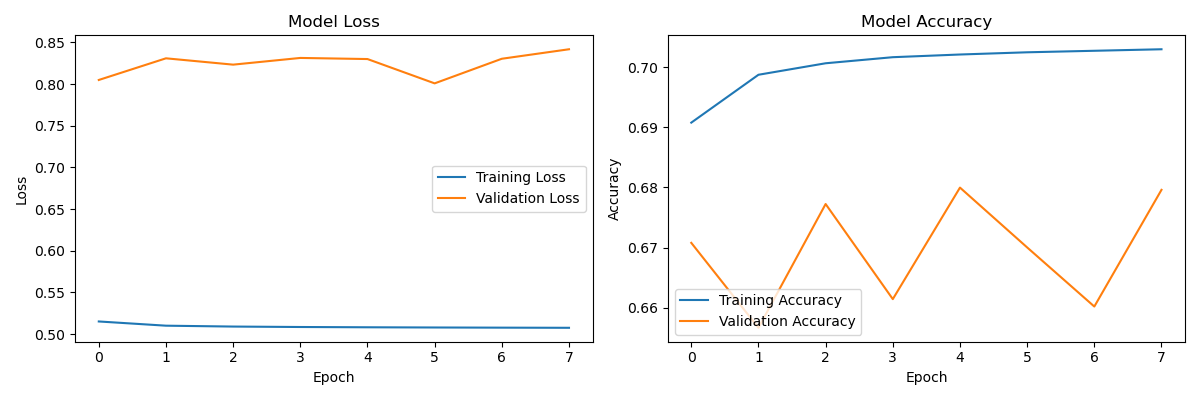
\includegraphics[width=\textwidth]{trainingstatistics/training_history_20250225_235938.png}
\caption{Training and validation metrics over training epochs.}
\label{fig:training_metrics}
\end{figure}

\subsection{LightGBM}
We used the LightGBM Python library to train and predict gesture segments. Unlike the CNN architecture, we consider only 2 labels here: \texttt{gesture} and \texttt{no-gesture} (\texttt{move} is merged into \texttt{no-gesture}). Videos are converted into sequences using the specified window size (5 by default). We use the World Feature set with 92 features. Feature extraction is detailed in \autoref{tab:lightgbm-feature-extraction}.

\subsubsection{Training}
As with the CNN model, we implement speaker-independent 3-fold cross-validation and run a hyperparameter search. Our search space considers num\_leaves between 31 and 63, max\_dept between 5 and 7, learning\_rate between 0.03 and 0.05, and class\_weight\_power between 0.5 (square root) and 1.0 (full inverse). In our tests, we identified the best hyperparameter combination as num\_leaves = 63, max\_dept = 7, learning\_rate = 0.05, and class\_weight\_power = 0.5. Since we have only 2 labels (\texttt{gesture} and \texttt{no-gesture}), we compare the predictions and ground truth to compute our metrics. For training, we continue until we have at least 200 trees. Early stopping is initiated when there is no improvement for 100 rounds. {\color{blue} We trained the model for up to 120 hours (the maximum time) on the Snellius National Supercomputer with an NVIDIA A100-SXM4-40GB GPU. Since we are still optimizing the model training procedure, we opted to limit the training time at 120 hours.}
We monitored the model's training progress through both loss and accuracy metrics on the training and validation sets. Figure~\ref{fig:training_metrics} plots the evolution of these metrics across training epochs, showing how both the training and validation loss decreased while accuracy increased over the 120-hour training period. The convergence of these curves indicates that our model successfully learned to classify gestures without significant overfitting.

\begin{table}[htbp]
  \caption{Feature Extraction}
  \label{tab:lightgbm-feature-extraction}
  \centering
  \begin{tblr}{
      width=0.98\textwidth,
      colspec={X[0.3,l] X[0.1,r] X[0.6,l]},
      row{1} = {font=\bfseries},
    }
    \toprule
    Feature Group & Count & Description \\
    \midrule
    Current pose	& 18 &	Key joint positions (shoulders, elbows, wrists) \\
    Velocity	& 18 &	Frame-to-frame joint velocities \\
    Wrist speeds	& 2 &	Left/right wrist speed magnitude \\
    Wrist ranges	& 6 &	Position range over window \\
    Finger positions	& 18 &	Pinky, index, thumb relative to wrist \\
    Finger distances	& 6 &	Inter-finger distances per hand \\
    Wrist acceleration	& 2 &	Left/right acceleration \\
    Trajectory smoothness	& 2 &	Velocity variation per wrist \\
    Wrist height	& 2 &	Height relative to shoulders \\
    Wrist spread	& 1 &	Distance between wrists \\
    Arm extension	& 2 &	Shoulder-to-wrist distances \\
    Total motion	& 1 &	Summed wrist displacement \\
    Symmetry features	& 2 & 	Position \& motion symmetry \\
    Visibility scores	& 20 &	Current, mean, and min visibility \\
    Total	& 100 &  \\
    \bottomrule
  \end{tblr}
\end{table}
% Results
\section{Results}
\label{sec:results}


\subsection{Testing Dataset}
For the testing dataset, we incorporated two recordings from MULTISIMO, one recording from the SaGA corpus, and one external recording of our own of a politician in the Irish Parliament, which we coded for gestures.

\subsection{Testing Metrics}
The EnvisionHGdetector's performance was evaluated using several complementary metrics. At the frame level, we employed standard classification metrics including weighted accuracy, precision, recall, and F1 score\footnote{Accuracy is the ratio of correct predictions to total predictions. Precision measures the proportion of correct positive predictions divided by the total number of positive predictions. Recall (also called sensitivity) measures the proportion of actual positives correctly identified. The F1 score is the harmonic mean of precision and recall, providing a balanced metric between false positives and false negatives.}. We also specifically track the false positive rate, which measures the proportion of non-gesture frames incorrectly classified as gestures, and false negative rate, the proportion of gesture frames incorrectly classified as non-gestures.

\subsection{Parameter Sensitivity Analysis}
Gestures are inherently continuous events, and we want users to be able to set their own parameters for tuning the gesture detection, next to the confidence thresholds for motion and gesture detection. The performance of the model is dependent on these thresholds. The model's performance was therefore systematically evaluated across four key parameters: the motion threshold (search space: 0.7, 0.8, 0.9, 0.95)\footnote{The motion threshold was not set for the entire stage as we discovered very early on that this needs be set to a high threshold in our early explorations.}, gesture confidence threshold (search space: 0.1, 0.2, 0.3, 0.4, 0.5, 0.6, 0.7, 0.8), minimum length in seconds of the gesture before it gets excluded (search space: 0.0, 0.1, 0.2, 0.3, 0.4), and minimum gap in seconds between similar labeled events for them to be not treated as one event (search space: 0.0, 0.2, 0.3, 0.4). We also assessed whether biasing the detection of co-speech gestures versus non-gestural ``move'' category increased performance (search space: 0.0, 0.1, 0.25). Since we are interested in the gesture classification performance, we ranked the best settings in terms of the F1 score for binary gesture classification. Thus, we aim to optimize for gesture, rather than (also) move classification. We first report the best parameter setting optimized for each dataset, and then the top-5 best global parameter settings, all ranked based on F1.



\begin{table}[htbp]
  \caption{Dataset-Specific Optimal Parameters and Performance (Optimized for Gesture F1 Score)}
  \label{tab:dataset-specific-parameters}
  \centering
  {\tiny
  \begin{tblr}{
      width=\textwidth,
      colspec={X[0.12,l] X[0.08,c] X[0.08,c] X[0.08,c] X[0.08,c] X[0.08,c] X[0.08,c] X[0.08,c] X[0.08,c] X[0.08,c] X[0.08,c]},
      row{1-2} = {font=\bfseries},
      rowsep=1pt,
      colsep=1pt
    }
    \toprule
    Dataset & Motion & Gesture & Min & Min & Gesture & Acc & Prec & Rec & F1 \\
    & Thresh & Thresh & Cert & Length & Class & & & & \\
    \midrule
    \textbf{CNN} \\
    \midrule
    External & 0.50 & 0.40 & 0.20 & 0.20 & 0.000 & 0.631 & 0.518 & 0.818 & 0.634  \\
    Multisimo & 0.50 & 0.40 & 0.00 & 0.00 & 0.00 & 0.974 & 0.566 & 0.583 & 0.573  \\
    SAGA & 0.50 & 0.30 & 0.00 & 0.00 & 0.25 & 0.832 & 0.815 & 0.898 & 0.854 \\
    \midrule
    Average & --- & --- & --- & --- & 0.083 & 0.812 & 0.633 & 0.766 & 0.687  \\
    \midrule
    \textbf{LightGBM} \\
    Dataset & LGBM & &  Min & Min & &  Acc & Prec & Rec & F1 \\
    & Thresh & & Cert & Length & & & & \\
    \midrule
    \midrule
    External & 0.50 & & 0.00 & 0.00 & & 0.453 & 0.411 & 0.915 & 0.567  \\
    Multisimo & 0.50 & & 0.00 & 0.30 & & 0.943 & 0.380 & 0.438 & 0.385  \\
    SAGA &      0.50 & & 0.00 & 0.40 & & 0.796 & 0.760 & 0.921 & 0.832   \\
    \midrule
    Average & --- & --- & --- & --- & --- & 0.731 & 0.517 & 0.758 & 0.595  \\
    \bottomrule
  \end{tblr}
  }
\end{table}


\begin{table}[htbp]
  \caption{Top 5 Parameter Combinations for all videos (Ranked by Gesture F1 Score)}
  \label{tab:top5-parameters}
  \centering
  {\tiny
  \begin{tblr}{
      width=\textwidth,
      colspec={X[0.1,c] X[0.1,c] X[0.1,c] X[0.1,c] X[0.1,c] X[0.12,c] X[0.12,c] X[0.12,c] X[0.13,c]},
      row{1-2} = {font=\bfseries},
      rowsep=2pt,
      colsep=2pt
    }
    \toprule
    Motion & Gesture & Min & Min & Gesture & Accuracy & Precision & Recall & F1 \\
    Thresh & Thresh & Cert & Length & Thresh & & & & \\
    \midrule
    \textbf{CNN} \\
    \midrule
    0.80 & 0.30 & 0.30 & 0.40 & 0.10 & 0.781 & 0.488 & 0.517 & 0.470 \\
    0.80 & 0.30 & 0.40 & 0.40 & 0.10 & 0.781 & 0.488 & 0.517 & 0.470 \\
    0.80 & 0.30 & 0.20 & 0.40 & 0.10 & 0.781 & 0.488 & 0.515 & 0.469 \\
    0.80 & 0.30 & 0.10 & 0.40 & 0.10 & 0.781 & 0.488 & 0.515 & 0.469 \\
    0.80 & 0.30 & 0.00 & 0.40 & 0.10 & 0.781 & 0.488 & 0.515 & 0.469 \\
    \midrule
    \textbf{LightGBM} \\
    \midrule
    0.80 & 0.30 & 0.30 & 0.40 & 0.10 & 0.781 & 0.488 & 0.517 & 0.470 \\
    0.80 & 0.30 & 0.40 & 0.40 & 0.10 & 0.781 & 0.488 & 0.517 & 0.470 \\
    0.80 & 0.30 & 0.20 & 0.40 & 0.10 & 0.781 & 0.488 & 0.515 & 0.469 \\
    0.80 & 0.30 & 0.10 & 0.40 & 0.10 & 0.781 & 0.488 & 0.515 & 0.469 \\
    0.80 & 0.30 & 0.00 & 0.40 & 0.10 & 0.781 & 0.488 & 0.515 & 0.469 \\
    \bottomrule
  \end{tblr}
  }
\end{table}

\subsection{Class-Specific Performance}
For a more detailed understanding, we compute these metrics separately for each class (\texttt{no-gesture}, \texttt{move}, and \texttt{gesture}) for the parameter set with the best global F1 score.
% Table 6: Per-Class Performance CNN
\begin{table}[htbp]
  \caption{Per-Class Performance (for Best Global Parameters)}
  \label{tab:class-performance}
  \centering
  {\small
  \begin{tblr}{
      width=0.95\textwidth,
      colspec={X[0.25,l] X[0.25,l] X[0.25,l] X[0.12,r] X[0.12,c] X[0.12,c] X[0.12,c]},
      row{1} = {font=\bfseries},
      rowsep=4pt,
      colsep=3pt
    }
    \toprule
    Class & Accuracy & Precision & Recall & F1 & FP Rate & FN Rate \\
    (Distribution) & & & & & & \\
    \midrule
    \textbf{CNN} \\
    \midrule
    None & 0.832 & 0.896 & 0.781 & 0.820 & 0.275 & 0.219 \\
    (73.5\%) & & & & & & \\
    \midrule
    Move & 0.958 & 0.177 & 0.309 & 0.224 & 0.024 & 0.691 \\
    (1.7\%) & & & & & & \\
    \midrule
    Gesture & 0.851 & 0.621 & 0.711 & 0.657 & 0.182 & 0.289 \\
    (24.9\%) & & & & & & \\
    \midrule
    \textbf{LightGBM} \\
    \midrule
    None & 0.788 & 0.880 & 0.692 & 0.742 & 0.347 & 0.308 \\
    (73.5\%) & & & & & & \\
    \midrule
    Move & 0.978 & 0.000 & 0.000 & 0.000 & 0.000 & 1.000 \\
    (1.7\%) & & & & & & \\
    \midrule
    Gesture & 0.784 & 0.482 & 0.674 & 0.541 & 0.320 & 0.326 \\
    (24.9\%) & & & & & & \\
    \bottomrule
  \end{tblr}
  }
\end{table}


\subsection{Gesture Frequency Tracking}

Finally, we cut each test video into 1 minute segments, and assess whether EnvisionHGdetector is a good solution for tracking gesture frequency (percentage time) over time. Below we use one of the top-5 settings to assess ground-truth and machine classification of gesture. We assess for each minute of video, the proportion of gestures as determined by the ground truth, which we then plot against the machine-labeled proportion of time gestured. These results indicate that there is a strong relationship (r = .90) between machine and human tracked gesture frequency, suggesting that the tool could be helpful for a computational approach to gesture rate tracking.
As shown in Figure~\ref{fig:segment-correlation}, there is a strong positive correlation ($r = .90$) between the ground-truth and machine-detected gesture percentages across one-minute video segments, demonstrating that EnvisionHGdetector reliably tracks relative gesture frequency even when individual gesture detection may not be perfect.

\begin{figure}[htbp]
  \centering
  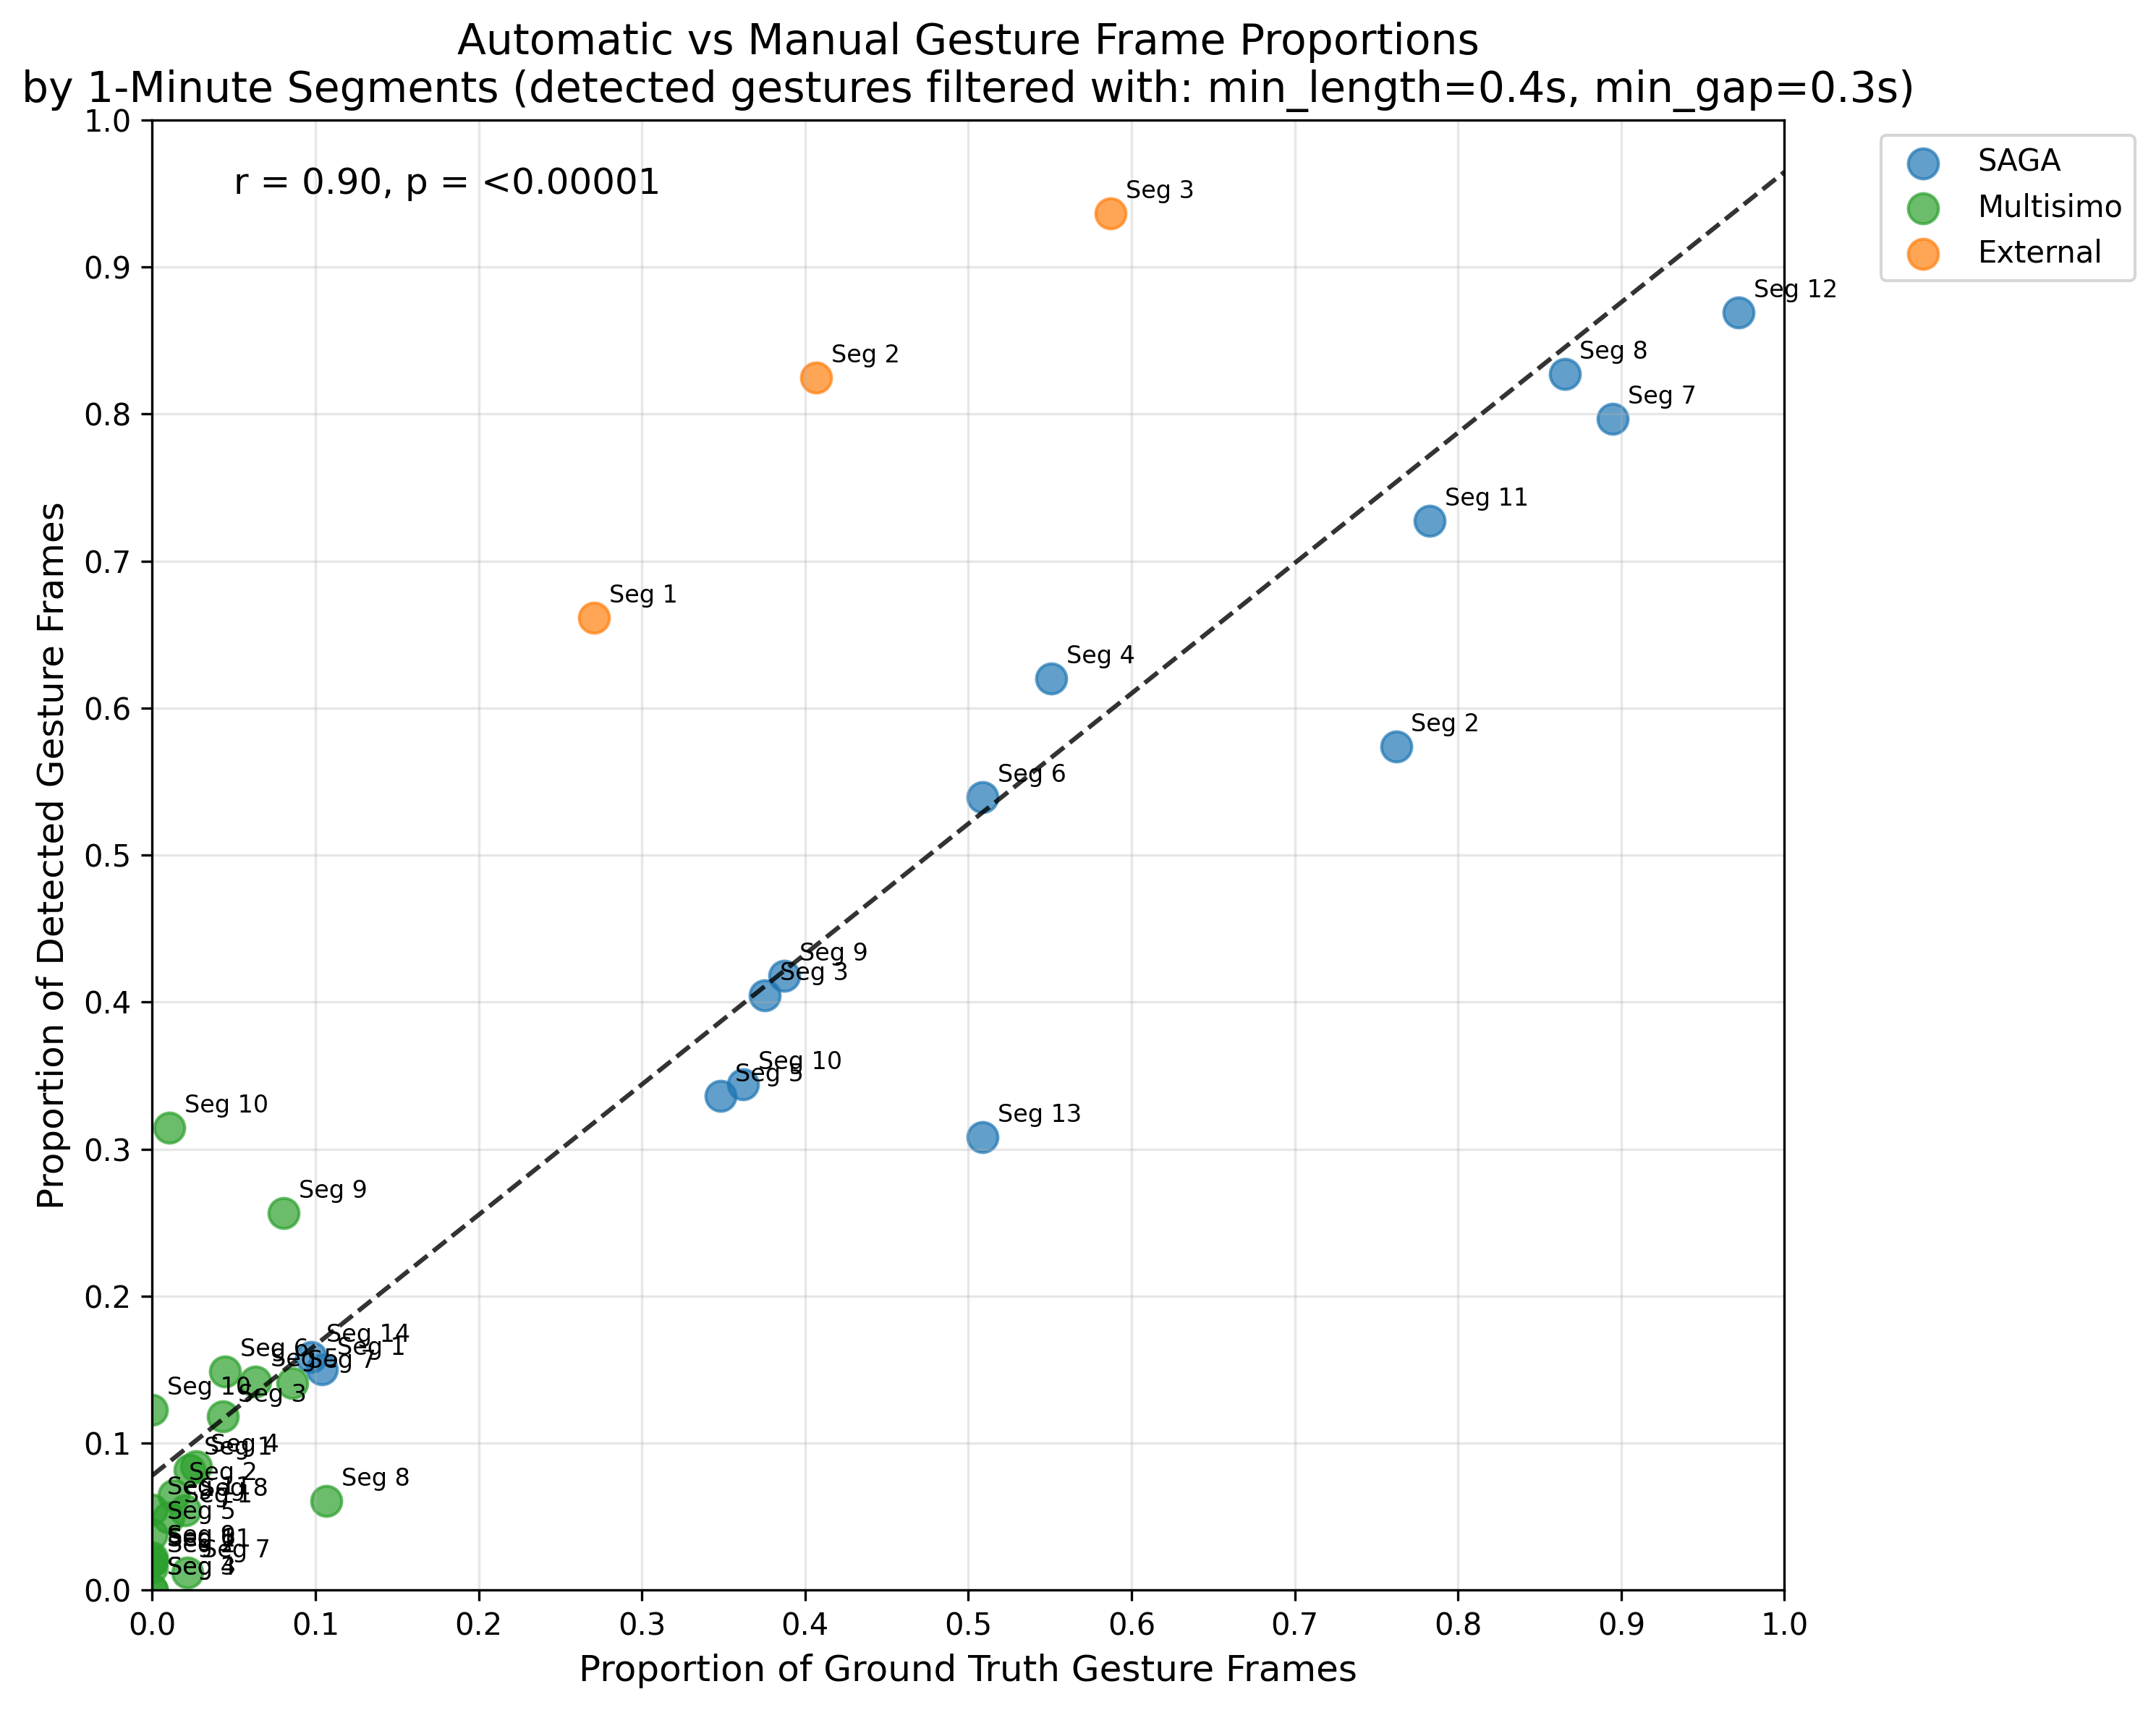
\includegraphics[width=0.98\textwidth]{recent_test_results/model2_withoutECOLANG/segment_correlation_by_1min.png}
  \caption{Co-speech gesture percentage tracking between ground-truth and machine labeled 1-minute segments}
  \label{fig:segment-correlation}
\end{figure}

\subsection{When Does Detection Fail? Gesture Subcategory Analysis}
The current classification is to be improved upon. To obtain a better understanding of what type of gestures fail to be tracked well, we can use the parts of test data that have specific gesture types annotated (namely SaGA and MULTISIMO). We observed that especially beat-like gestures are difficult to track, while pure iconic, discourse, and deictic gestures were (relatively) easier to track. This provides important information that the current model is more sensitive towards classifying iconic gestures. This is possibly because iconic gestures are often for showing something depictively, and thus involve more elaborate and visually salient trajectories that have longer durations. In other words, these gestures are less difficult to miss by the classifier. Figure~\ref{fig:difficulty_ranking} quantifies this relative detection difficulty for each gesture subcategory by displaying their difficulty ratings (calculated as 1$-$F1 score).

\begin{table}[htbp]
  \caption{Detailed Performance by Gesture Category (Sorted by F1 Score)}
  \label{tab:gesture-performance}
  \centering
  {\small
  \begin{tblr}{
      width=\textwidth,
      colspec={X[0.18,l] X[0.18,l] X[0.12,c] X[0.12,c] X[0.12,c] X[0.17,r] X[0.17,r]},
      row{1} = {font=\bfseries}
    }
    \toprule
    Category & Precision & Recall & F1 & Accuracy & Frame Count & \% of Total \\
    \midrule
    discourse & 0.148 & 0.489 & 0.227 & 0.591 & 2,497 & 20.7\% \\
    iconic & 0.157 & 0.514 & 0.216 & 0.808 & 4,944 & 41.1\% \\
    deictic & 0.139 & 0.477 & 0.215 & 0.588 & 2,406 & 20.0\% \\
    iconic-beat & 0.046 & 0.572 & 0.086 & 0.598 & 669 & 5.6\% \\
    iconic-deictic & 0.043 & 0.424 & 0.078 & 0.587 & 837 & 7.0\% \\
    beat & 0.042 & 0.443 & 0.074 & 0.784 & 455 & 3.8\% \\
    symbolic & 0.029 & 0.756 & 0.054 & 0.879 & 49 & 0.4\% \\
    deictic-beat & 0.008 & 0.441 & 0.016 & 0.592 & 152 & 1.3\% \\
    other & 0.000 & 0.000 & 0.000 & 0.592 & 25 & 0.2\% \\
    \bottomrule
  \end{tblr}
  }
\end{table}


\begin{figure}[H]
\centering
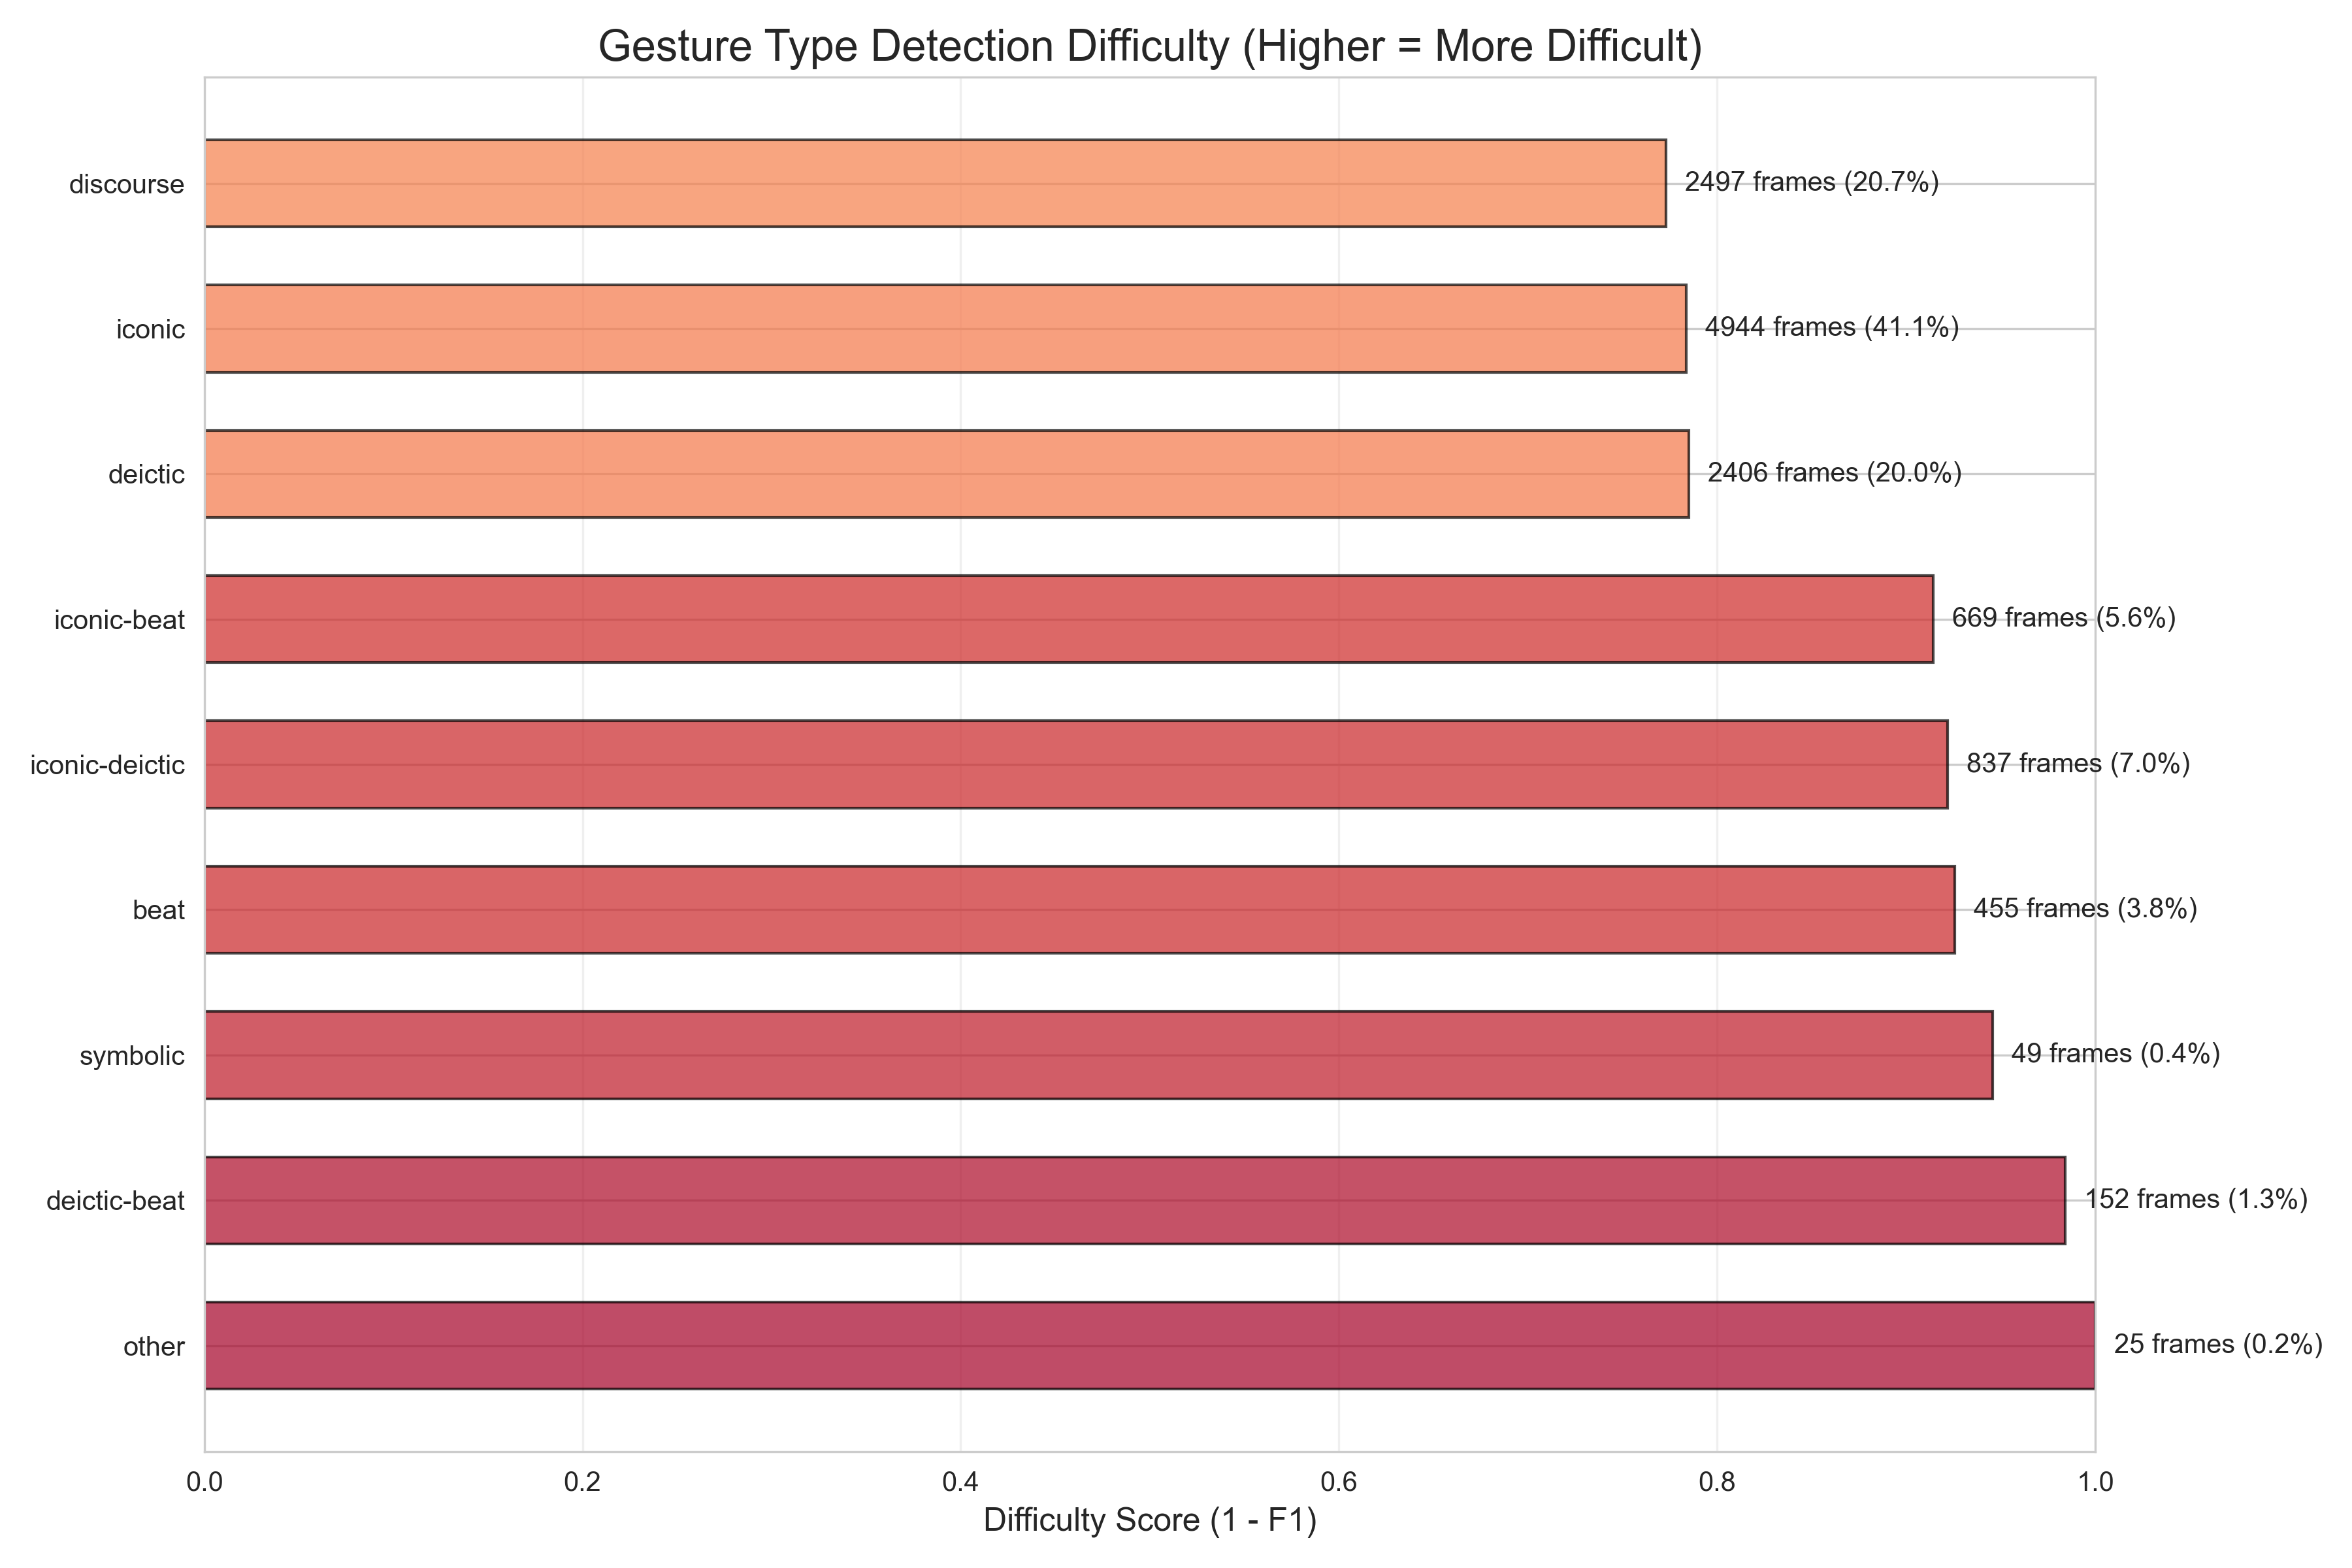
\includegraphics[width=\textwidth]{gesture_difficulty_ranking.png}
\caption{The difficulty ratings (1$-$F1) for the classifier to label a co-speech gesture when the ground truth had this type of gesture sub-category label. These labels were based on SaGA and MULTISIMO.}
\label{fig:difficulty_ranking}
\end{figure}



\subsection{EnvisionHGdetector Package Details}
We have released the EnvisionHGdetector software as a Python package (recommended for Python 3.9), including the most recently trained CNN model, on \href{https://pypi.org/project/envisionhgdetector/}{PyPi}, which allows for an easy \texttt{pip}-based install of the package into a Python environment. The code is open source and is available in a \href{https://github.com/WimPouw/envisionhgdetector}{GitHub repository} \parencite{pouwEnvisionhgdetectorHandGesture2024}. The \href{https://envisionbox.org/embedded_UsingEnvisionHGdetector_package.html}{EnvisionBOX website} provides a Jupyter notebook detailing the use of the EnvisionHGdetector with the CNN that we report here as part of version 1.0.0 with sample data input. This notebook and repository will also be continuously updated with the most recent package methods.

\subsubsection{Gesture Detection}
The package employs the trained model in a sliding window fashion on the skeleton feature data for an entire video, with a window length of 25 frames and step length of 1 frame. The label confidences are then assigned to the middle frame of the window. One can further tune the detector to more liberally recognize movements and gestures (increasing false positive rates but reducing false negative rates) or be more conservative (increasing false negative rates but reducing false positive rates). One may further specify what the minimal length should be of a detected gesture (minimal gesture length in seconds) and when gestures with short gaps need to be merged as a single gesture (minimum gap size in seconds). The user can further increase the likelihood that a gesture is detected at the expense of categorizing a non-gestural movement. For the current version of the EnvisionHGdetector package, we recommend the input videos to have 25 to 30 fps, so that it corresponds to the training dataset. However, our tool incorporates a downsampling strategy if the video has a higher fps.

The EnvisionHGdetector software further provides utility functions that create outputs, including a CSV file with frame-by-frame confidence predictions for gesture and motion, a CSV file of segmented gesture intervals, a NumPy file of the extracted features for each detected gesture, and importantly also a labeled video with real-time gesture annotations overlaid (an example is \href{https://osf.io/e4drq}{available online}). Adopting a similar approach to \citet{ienagaSemiautomationGestureAnnotation2022}, we also generate ELAN annotation files compatible with gesture studies annotation workflows. In the following, the additional kinematic analysis pipeline functions are described.

\subsubsection{Retracking and Kinematic Analysis}
\emph{Retracking.}
A common issue in conducting motion analyses using video-based motion tracking is that pose positions are often provided in pixels, typically in 2D, which complicates comparisons across videos with varying video-recordings and body-to-camera angles. To increase generalizability, we therefore implement an option that allows retracking the gestures with pose landmarks estimated in metric space, using MediaPipe's pose world landmarks. This can only be generated for the body keypoints (and not for the hand or face features). After retracking, for each gesture, the tool provides the metric-scaled 3D skeleton data, as well as the tracked video with skeleton imposed to assess tracking quality further.

\emph{DTW.} 
After retracking the gesture segments, one can then invoke a kinematic analysis pipeline, beginning with creating a Dynamic Time Warping \parencite{giorginoComputingVisualizingDynamic2009} dissimilarity matrix, as proposed by \citet{pouwGestureNetworksIntroducing2019}. To do this, we rely on Shape-DTW \parencite{zhaoShapeDTWShapeDynamic2016} with the \href{https://github.com/MikolajSzafraniecUPDS/shapedtw-python}{Python package} shapedtw \parencite{szafraniecMikolajSzafraniecUPDSShapedtwpython2025}. Shape-DTW enables the comparison of multidimensional time series using non-linear time warping, similar to classic DTW \parencite{giorginoComputingVisualizingDynamic2009a}. It also provides a method to incorporate more context from the matched indices of the query and reference time series. A tutorial regarding the application to gestural data is available.\footnote{See \url{https://envisionbox.org/embedded_Gesture_kinematic_spaces.html}}

Following the procedure as outlined in \citet{pouwGestureNetworksIntroducing2019}, for all gestures \( N \), we compute for each combination of gesture \( i \) versus gesture \( j \), a Shape-DTW normalized distance based on the position time series of the upper limbs (left and right shoulders, elbows, wrists, pinkie fingers, indices, and thumbs). The warping path was determined by taking in a context of the raw subsequence width of 160 ms (4 indices) applied on the multidimensional time series of the upper limbs trajectories. As such, the current approach is a multidimensional dependent variant of dynamic time warping \parencite{giorginoComputingVisualizingDynamic2009}. A symmetric distance matrix \( D \) with \( i \) rows and \( j \) columns, where \( D_{ij} \) = 0 on the diagonals, i.e., when \( i = j \). The distance \( D \), is then filled capturing each kinematic similarity for each gesture comparison and saved as output by EnvisionHGdetector. The package also saves a dimensionality reduced representation of  \( D \), by applying UMAP on \( D \), reducing the space to two dimensions \parencite{mcinnesUMAPUniformManifold2020}. This dimensionally reduced representation is then later optionally used for data visualization of the kinematic (dis)similarity space.

\emph{Kinematic Analysis.} 
For each gesture we extract from the Gaussian smoothed time series, a comprehensive set of features is calculated on the most active hand of the gesture (i.e., left or right), adapted from \href{https://envisionbox.org/embedded_Analysis_kinematic_features_module.html}{EnvisionBOX} and discussed and tested in depth in a study by  \citet{trujilloMarkerlessAutomaticAnalysis2019}. An overview of the features is given in Table 8. EnvisionHGdetector then generates a flat dataset for each gesture observed, and all their accompanying features. Such a flat dataset can then be aligned with metadata and used for statistical analyses, e.g., comparing peak velocity for different speakers; assessing gesture prominence across time; see e.g., \citet{rasenbergMultimodalNatureCommunicative2022, pouwSystematicInvestigationGesture2021, trujilloCommunicativeIntentModulates2018}. 

\emph{Dashboard Visualization.} 
After kinematic analyses, another function may be invoked to generate a dynamic data dashboard, which allows for an interactive data visualization using the generated kinematic analysis output. The dashboard is created as a separate Python script, which runs a local server, or can be run on a server as exemplified 
\href{https://tsg-131-174-75-200.hosting.ru.nl/envisionhgdetectordashboard/}{online} (our server-ready dashboard runs on an Apache2-supported server). The Dashboard uses Plotly Dash and dynamically links the retracked videos with the kinematic dissimilarity space, as well as the kinematic features results. By selecting individual points in the kinematic space or the jitter points in the kinematic feature violin/boxplot/jitter plots, the user can inspect the original video data against the quantitative output. Figure~\ref{fig:eg_pipeline} presents the interactive dashboard visualization snapshot. The dashboard allows researchers to explore the kinematic relationships between detected gestures, enabling direct video playback of selected gestures for qualitative assessment alongside quantitative metrics.

\begin{figure}[H]
    \centering
    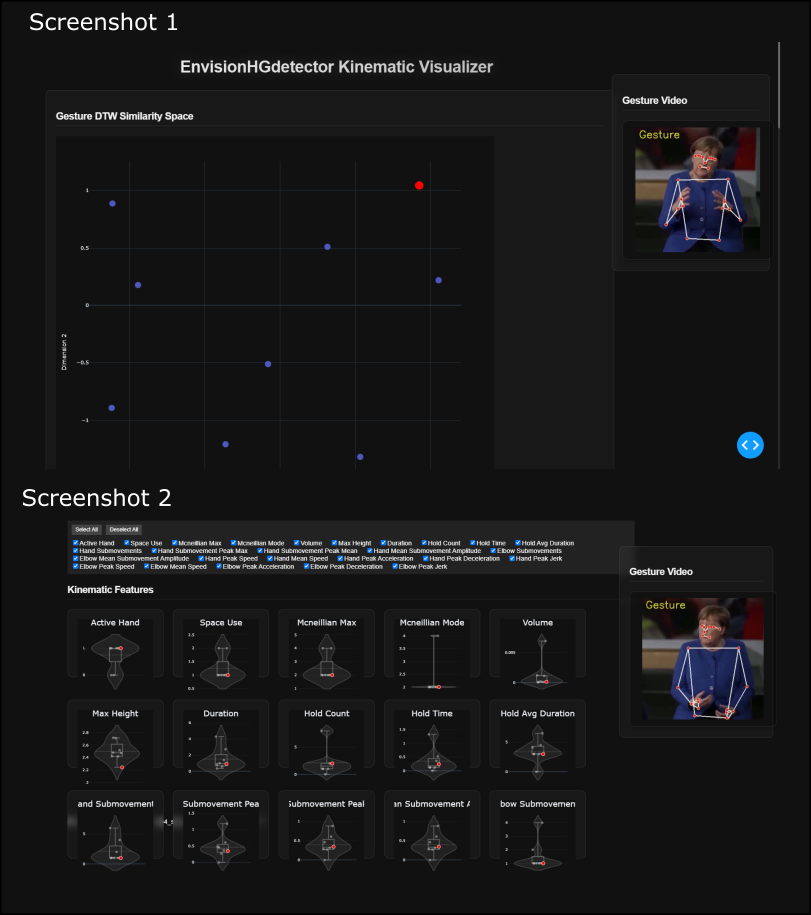
\includegraphics[width=0.98\linewidth]{exampledashboard.png}
    \caption{Sample visual of the visualization dashboard. Screenshot 1 shows the UMAP space of the gesture similarity spaces that is based on the DTW distances between all gesture pairs. Closer points in space indicate more kinematically similar gestures. Screenshot 2 shows the element under the similarity space, containing for all gestures the distribution of kinematic features. By selecting any of the individual points in the jitter plot or the similarity plot, the data point is highlighted and the detected gesture played. A live server version of the dashboard using example data is \href{https://tsg-131-174-75-200.hosting.ru.nl/envisionhgdetectordashboard/}{available online}.}
    \label{fig:eg_pipeline}
\end{figure}



% Table 8: Kinematic Features Overview
\begin{table}[htbp]
  \caption{Kinematic Features Overview}
  \label{tab:kinematic-features}
  \centering
  {\small
  \begin{tblr}{
      width=\textwidth,
      colspec={X[0.3,l] X[0.7,l]},
      row{1} = {font=\bfseries},
      cell{2}{1} = {c=2}{l},
      cell{4}{1} = {c=2}{l},
      cell{9}{1} = {c=2}{l},
      cell{14}{1} = {c=2}{l},
      cell{19}{1} = {c=2}{l},
      rowsep=1.5pt,
      stretch=0.85
    }
    \toprule
    Feature Category & Description \\
    \midrule
    \textit{Hand} & \\
    Active hand & The most active hand for this gesture \\
    \midrule
    \textit{Spatial Features} & \\
    space use & Number of distinct spatial zones used by the active hand in McNeillian space \\
    mcneillian max & Maximum zone reached by each hand (1=center-center to 4=extreme periphery) \\
    volume & 3D volume covered by the active hand \\
    max height & Maximum vertical height reached by the active hand (0–5 scale) \\
    \midrule
    \textit{Temporal Features} & \\
    duration & Total gesture duration in seconds \\
    hold count & Number of detected gesture holds \\
    hold time & Total time spent in holds (seconds) \\
    hold avg duration & Average duration of holds \\
    \midrule
    \textit{Submovement Features} & \\
    hand submovements & Total number of submovements for the active hand \\
    hand mean submovement amplitude & Average amplitude of hand submovements \\
    elbow submovements & Number of distinct elbow submovements \\
    elbow mean submovement amplitude & Average amplitude of elbow submovements \\
    \midrule
    \textit{Dynamic Features} & \\
    hand peak speed & Maximum speed reached by the active hand (meters/s) \\
    hand mean speed & Mean speed of the active hand (meters/s) \\
    hand peak acceleration & Maximum acceleration/deceleration of the active hand (meters/s²) \\
    hand peak jerk & Maximum rate of change of hand acceleration (meters/s³) \\
    elbow peak speed & Maximum speed reached by the active elbow (meters/s) \\
    elbow mean speed & Mean speed of the active elbow (meters/s) \\
    elbow peak acceleration & Maximum acceleration/deceleration of the active elbow (meters/s²) \\
    elbow peak jerk & Maximum rate of change of elbow acceleration (meters/s³) \\
    \bottomrule
  \end{tblr}
  }
\end{table}


% Discussion
\section
{Discussion}
\label{sec:discussion}
We have introduced the first version of the EnvisionHGdetector, which allows for simple classification of co-speech gesture, non-gestural movement (self-adaptors, object manipulations), and a neutral category, referred to as no-gesture events. The toolkit further allows for kinematic feature analysis and kinematic similarity analysis using DTW, which is dynamically visualized in a dashboard that links to the tracked gesture segments. 

We obtained for the gesture classification that the CNN-based detector using input from MediaPipe Holistic for extracting pose features attains an accuracy of 73-78\% and an F1 score of .496 to .541 on unseen data. The performance is encouraging, but not perfect. For example, it is not reaching performance levels reported on custom-trained models on specific datasets \parencite{ienagaSemiautomationGestureAnnotation2022, ghalebCoSpeechGestureDetection2024}. However, the current model performs reasonably well across samples from a variety of different datasets, even from completely external sources. The current model also has much lower false positive rates (21\% to 33\%) as compared to rule-based detection based on movement speed \parencite{pouwSemanticallyRelatedGestures2021, ripperdaSpeedingDetectionNoniconic2020} (70–86\%), because we also train the model on non-gestural movement events and gesture events. Our results also show a false negative rate of .36\% to 48\%, which can be improved upon. Our results show that especially beat gestures were difficult to detect, which are often short and rapid. Symbolic gestures were also tracked less well, which is intuitive, as they contain little movement and rather consist of hand postures. Importantly, the current model seems to very reliably track gesture rate (r = .90), which makes us confident that EnvisionHGdetector may prove a very valuable tool for large-scale investigation of co-speech gesture rates or analyses that do not depend on capturing every gesture instance (e.g., focusing on summary characteristics between individuals, populations, or contexts). Given the unique training dataset and the light-weight nature of the current tool that can be used on normal consumer laptops without GPU support, we believe that this gesture detection tool can be valuable for a variety of research projects. 

\subsubsection{Usage Advice \& Workflow}
We envision that the current tool is more valuable for some applications than others. In general, we think tools like these should not, and will not, replace human annotation practices in gesture studies. For some projects, one clearly needs human-level performance of gesture detection with proper boundaries for strokes. For example, since the current models take in 25 frames, they tend to have larger gesture segments, with multi-stroke units. But even in cases where there are high precision requirements, annotations likely speed up the process of identifying potentially relevant events \parencite{ripperdaSpeedingDetectionNoniconic2020}. There are also projects where such coding-scheme-dependent precise annotations are not needed. Many kinematic analyses require only some isolation of gestural movements as to then capture kinematic features, e.g., in gesture–speech coupling \parencite{wagnerGestureSpeechInteraction2014}, or kinematic correlates informative for effort \parencite{rasenbergMultimodalNatureCommunicative2022}, or clustering of recurrent gestures \parencite{mcneillCatchmentsProsodyDiscourse2001, beecksSpatiotemporalSimilaritySearch2015}. For example, if one is interested in the role of gesture acceleration relative to F0 change in speech, one can use automatic sampling of gestures and moments of speech, and their relationship -- given enough data and further filtering based on acoustics and kinematics -- should be tolerable towards false positive or false negative gesture identification. Furthermore, if one wants to have a computationally reproducible way to track gesture frequency, we believe this tool is sufficiently reliable to track obvious differences \parencite{hogrefeActualPotentialUse2013}. In all such cases, automatic annotation tools such as the current one will help to drastically scale up the analyses that are currently typical in the field.

In terms of using this tool, we do have several points of advice. If using this tool to track gesture frequency, we recommend that the recording conditions be comparable across recordings. We also advise to use the tool on videos recorded at 25/30 fps, where a single person is visible. Since pose tracking can be affected when the person is interacting with objects, we presume that the tool will work better if the subjects are not holding objects while they are speaking. Of course, the goal of our project is to overcome these constraints that might affect usability.

Once data is collected, an example pipeline for applying the envisionHGdetector can be as follows:
\begin{itemize}
\item Determine if the project calls for more \textit{conservative} (more data, more noise) or more \textit{liberal} (less data, less noise) gesture sampling
\item Run EnvisionHGdetector on one video
\item Manually check annotations to determine if the detection quality is acceptable
\item Proceed processing the rest of the dataset, or revise model parameters (e.g., gesture threshold)
\item For more precise results, manually remove false positive annotations (e.g., in ELAN\footnote{\url{https://archive.mpi.nl/tla/elan}})
\item Use dashboard visualizations to further check and/or explore data 
\item Proceed with statistical analyses (e.g., gesture rate, kinematics), by loading in the gesture segment data, dissimilarity distance matrix, or kinematic feature flat data frames in one's analysis software of choice (including R, Python, SPSS).
\end{itemize}

\subsubsection{Strengths \& Limitations}
The current model behind EnvisionHGdetector (v1.0.0.1) was trained on openly available datasets with gesture annotations. It possesses broad generalizability in the sense that it was trained on several varied datasets, but still this does not mean that the training set was truly sufficiently varied. For example, most of the datasets, except TEDM3D \parencite{rohrerTemporalPragmaticAnalysis2022}, were based on experimental contexts or standard front-view camera angles. This means that our current model will likely not perform that well on challenging video datasets with changing camera angles or frame cuts. However, it should be noted that the datasets did contain spontaneous gestures, rather than scripted or prompted gestures, which increases the relevance of this tool for researchers interested in spontaneous co-speech gestures. There are likely other such sources of variability that we are missing, and therefore our goal for creating an out-of-the-box solution for researchers needs to be weighed against the limitations of the limited amount of currently open datasets that contain gesture annotations by expert gesture researchers. In sum, while our model is trained on much more variable and large datasets than previously trained models on single-sourced training data, we acknowledge that variability in the training data could be much improved. We thus encourage more work in gesture detection leveraging not just designed data (experimental setups), but also organic data (video data in the wild available outside of academic settings).

A further problem relating to the lack of variability is the set of spoken languages under which gestures were produced. Gesture production varies substantially across cultural and linguistic contexts, raising questions about cross-cultural generalizability. English, French, Chinese, and German are currently present in the training data. Languages and cultural contexts absent from the training data might therefore present challenges, mainly if they employ distinct gesture spaces or stereotypical gestures. Expanding the training data to encompass greater cultural diversity represents an important direction for future development.

Next to a lack of variability, there is paradoxically also too much variability in the training dataset. Namely, each research team that generated the original gesture corpora and datasets each had their own unique gesture labels and gesture annotation strategies that are definitely implicitly present, or are indeed explicitly reported upon. For example, for the TEDM3D \parencite{rohrerTemporalPragmaticAnalysis2022} data, we noticed that the stroke annotations were extremely short, while for MULTISIMO \parencite{koutsombogeraMULTISIMOMultimodalCorpus2017}, gesture strokes were more liberally extended into multiphase movements. This may be in part due to differences in genre, but likely also due to mere differences in annotation practices. Indeed, the parsing of continuous stream of gestures into single or multi-unit strokes is one of the most difficult aspects for human annotators. However, this presumed variability in human ground truth annotation in our training data can be a curse or a blessing depending on how you look at it. There are many ways to parse a gesture, and we assume that the current model makes estimates based on trying to satisfy different annotation strategies that underlie the training data. 

In our testing metrics, we have not yet at this stage incorporated other types of performance metrics often used in gesture studies. In general, we could argue that more testing needs to be done to argue for widespread usability. The current project is work in progress and we hope to expand on this with more training data and more robust models. At the same time, tools like the current one, regardless of performance metrics advertised, will need to prove their value in practice. To increase use value, the EnvisionHGdetector provides means to produce ELAN files that can easily be used in computing field-specific annotation agreement metrics. We hope that the tool can also be more widely tested according to the field-specific standards.

A strength of EnvisionHGdetector is that it is the first tool of its kind that provides automatic kinematic analysis, much like an OpenSmile feature processing routine \parencite{eybenOpensmileMunichVersatile2010}, but for gesture. For each gesture, the software provides metric-scaled information about speed, acceleration, sub movements, and other types of features that have been used to qualify gestures by reseachers \parencite{trujilloMarkerlessAutomaticAnalysis2019, trujilloCommunicativeIntentModulates2018, pouwSystematicInvestigationGesture2021}. It also generates embedding spaces of all the gestures produced, as proposed in the gesture network approach, which takes advantage of DTW \parencite{pouwGestureNetworksIntroducing2019}. Indeed, we believe that this will increase the potential usability of more computational signal processing pipelines that are now only sparingly applied in the field. Importantly, for most computational research on gestures, the gesture annotation phase has always been an important bottleneck for scaling up to a more widespread computational study of multimodal behavior. This scaling up is needed if we want to come to generalizable answers to some classic questions in the field, such as, when do we gesture; are gestures different for different cultures, and many more. Having said this, we also believe, of course, that many research questions in the field do not require an automatic detection tool like the current one.

The computational demands of gesture analysis vary significantly based on hardware specifications. Consumer laptops using CPU-only processing might require 2–3 times the video duration for analysis, making them suitable for smaller projects under 10 hours of video. Mid-range desktops might process at 1.5–2 times video duration, while high-end workstations could approach real-time processing rates. GPU acceleration could potentially achieve sub-real-time processing (0.2–0.5× video duration), enabling large-scale corpus analysis. These considerations suggest that while the tool is accessible to researchers with standard computing resources, significant efficiency gains could be realized through hardware optimization for large-scale projects.

\subsubsection{Future Outlook}
With this paper, we also emphasize the need for more openly available datasets for the development of computational methods in social science. Gesture is a vital part of human communication, not a rare commodity. Yet, due to (much needed) limitations for privacy protection, and at the same time also due to the slow adoption of progressing norms in (open) science \parencite{resnikShouldResearchersDestroy2024}, we still lack a benchmarked, highly varied gesture-annotated dataset of human co-speech gestures. Therefore, we are currently curating and considering different masking techniques \parencite{owoyeleMaskedpiperMaskingPersonal2022,owoyeleMaskAnyoneToolkitOffering2024} to generate a fully (retrackable) de-identified gesture dataset comprising over 16,000 annotated instances that can be easily used as a co-speech gesture benchmark dataset. Such a dataset would provide a valuable resource for training models with improved communicative action recognition performance.

 Several promising research directions could enhance gesture detection capabilities and applicability. Future work might explore alternative architectural approaches beyond our CNN implementation. While the current architecture was selected for its balance of performance and efficiency, other architectures such as 
 LSTMs \parencite{shahroudy2016skeleton}, 
Graph Convolutional Networks \parencite{yan2018stgcn, liu2020dcgcn}, or Transformer-based models \parencite{girdhar2019video, jiang2022inception} could potentially offer different advantages, particularly for capturing long-range temporal dependencies or structural relationships between body parts. The computational requirements for such architectures would likely increase significantly, needing careful evaluation of the quality–efficiency tradeoff. Additionally, newer machine learning models architectures are sometimes pre-retrained on large action class datasets, which may further yield much better gesture performance levels (after retraining) \parencite{zhuMotionBERTUnifiedPerspective2023}.


Once satisfying performance is obtained in co-speech gesture detection, obvious future projects that spring from the current one are training similar models on different gesture types. This does limit the use of some datasets due to label practice mismatches. Nevertheless, with MULTISIMO \parencite{koutsombogeraMULTISIMOMultimodalCorpus2017} and SaGA data \parencite{luckingBielefeldSpeechGesture2010} in hand, one could train a gesture type classifier by differentiating beat, iconic, deictic gestures, or perhaps a classifier that allows for some dimensionality, where a beat gesture can be an iconic gesture, too, for example \parencite{rohrerTemporalPragmaticAnalysis2022}. 

Additionally, improvements of the current work could arise from a reevaluation of the feature set. It has for example been shown that adding speech features may improve gesture classification \parencite{ghalebLeveragingSpeechGesture2024}. Understanding the relative contribution of different feature sets through ablation could guide future refinements of the model. For example, we hypothesize that hand features contribute most significantly to model performance, while facial features play a less critical role. A systematic ablation study could test these hypotheses by progressively removing feature groups and measuring the impact on detection accuracy offering opportunities to streamline the feature set without compromising performance, potentially improving computational efficiency.

Adopting computational tools such as EnvisionHGdetector within the gesture research community likely depends on several factors beyond raw performance metrics. Technical accessibility, workflow integration with existing annotation tools, interpretability of detection decisions, customizability for specific research questions, and compatibility with analysis software all influence usability. Future user studies could explore these dimensions to better align tool development with researcher needs across different subdisciplines, including linguistics, psychology, and human-computer interaction.

\subsection{Conclusion}
 The current EnvisionHGdetector represents a crucial step toward generalizable co-speech gesture detection and standardized kinematic analysis and visualization. While the current detection capabilities await further improvements, we believe that the current toolkit will already open up new research avenues, specifically promising to increase analysis capabilities of large datasets that are not possible to  annotate by hand. 
Future research should, however, systematically investigate potential disparities in model performance across demographic groups underrepresented in training data, cultural contexts with distinct gesture conventions, neurodivergent populations with potentially divergent gesture patterns, and varying recording environments. We propose that as this field advances, standardized benchmark datasets representing diverse populations should enable a more rigorous evaluation of algorithmic fairness in gesture detection.


\begin{comment}
    \begin{figure}[htbp]
  \centering
  \includegraphics[width=0.5\textwidth]{example-image-a}
  \caption{A}
  \label{fig:a}
\end{figure}
\end{comment}



%% References:
\clearpage
\printbibliography[heading=subbibliography]
\end{refsection}
\end{document}


%%% Local Variables:
%%% mode: latex
%%% TeX-master: t
%%% End:
